\documentclass[11pt, oneside]{article}   	% use "amsart" instead of "article" for AMSLaTeX format
\usepackage{geometry}                		% See geometry.pdf to learn the layout options. There are lots.
\geometry{letterpaper}                   		% ... or a4paper or a5paper or ... 
%\geometry{landscape}                		% Activate for rotated page geometry
%\usepackage[parfill]{parskip}    		% Activate to begin paragraphs with an empty line rather than an indent
\usepackage{graphicx}				% Use pdf, png, jpg, or eps§ with pdflatex; use eps in DVI mode
								% TeX will automatically convert eps --> pdf in pdflatex		
\usepackage{amssymb}

%SetFonts
\graphicspath{ {./images/} }
%SetFonts

\usepackage{caption}
\captionsetup[figure]{labelformat=empty}%
\usepackage{subcaption} 

\usepackage{amsmath}


\title{Crittografia}
%\author{The Author}
\date{}							% Activate to display a given date or no date
\usepackage{float}
\begin{document}
\maketitle
%\section{}
%\subsection{}
Programma:
\begin{itemize}
\item Accenni storici
\item Cifrario simmetrico con una chiave
\item Cifrario asimmetrico con due chiavi, una per aprire una per chiudere
\item Funzioni hash
\end{itemize}


\long\def\comment#1{
\section*{Domande da fare al prof}
\begin{itemize}
\item Abbiamo detto che nella XTS o XEX enconding scheme non possiamo utilizzare una cifratura a $2^{256}$ perché 256 non è un numeor primo, perchè?
\item Cos'è la proprietà di delta set, in essenza?	ok
\item anki common modulus attack, low exponent to do
\item come funziona il bit commitment?	ok
\item $k$ casuale segreto di elgamal		ok
\end{itemize}
}

\section*{Cifratura simmetrica e cifratura asimmetrica}
L'obbiettivo fondamentale della crittografia è permette a due persone, solitamente chiamate Alice e Bob di comunicare su un canale di comunicazione insicuro, facendo in modo che un attaccante, solitamente chiamato Eve, possa intercettare il messaggio.\\
I canali di comunicazione possono essere molteplici (internet, telefono etc.). Il messaggio inviato da Alice è chiamato plaintext, un testo in inglese di struttura arbitraria. Alice cifra il messaggio utilizzando una chiave, e spedisce il ciphertext lungo il canale di comunicazione a Bob, che decifra il messsaggio e ricostruisce il plaintext.\\

I cifrari che andiamo a vedere sono suddivisi in cifrari:
\begin{itemize}
\item simmetrici, in cui la chiave di cifratura è uguale alla chiave di decifrazione. I cifrari simmetrico vengono utilizzate per cifrari grosse quantità di dati (eg. testo, \emph{des e aes})
\item asimmetrici, in cui la chiave di cifratura è diversa dalla chiave di decifrazione. I cifrari asimmetrici vengono utilizzati per cifrare piccole quantità di dati (eg. pw, \emph{rsa, elgamal})
\end{itemize}
Dobbiamo infine accennare le tecniche steganografiche, che sono tecniche di offuscazione del messaggio

\subsection*{Sicurezza di un cifrario}
Uno dei principali obbiettivi di un cifrario è sicuramente la sicurezza, ma come facciamo a quantificarla? Generalmente possiamo dire che un cifrario è sicuro se un attaccante non riesce a decifrare il messaggio senza una chiave. \\Uno dei principi che i cifrari seguono maggiormente è il principio di Kerkhoff.
\subsection*{Principio di Kerkhoff}
Il principio di Kerkhoff ci dice di assumere che l'attaccante conosca sempre l'intero schema/protocollo e la chiave pubblica, ma non la chiave privata (security through obscurity non funziona).\\
\emph{Brutalmente: se un cifrario rimane pubblico per 30 anni, ma non viene bucato, vuol dire che è resiliente}
\subsection*{Scenari di attacco}
I principali modelli di scenario di attacco sono:
\begin{itemize}
\item known ciphertext only, in cui l'avversario conosce una porzione del cyphertext
\item known plaintext, in cui l'avversario conosce una porzione del plaintext, e ha accesso al relativo ciphertext
\item chosen plaintext, in cui l'attaccante è in grado di scegliere un plaintext, e possiede il relativo ciphertext
\item chosen cypher-text, in cui l'attaccante è in grado di scegliere il ciphertext, ed è poi fornire del plaintext
\end{itemize}
Chiaramente gli attacchi chosen plaintext e chosen ciphertext sono gli attacchi che forniscono più informazioni ad un potenziale attaccante.
\section*{Le proprietà delle funzioni crittografiche}
Vi sono una serie di proprietà che devono garantire delle funzioni crittografiche perché siano considerabili, ovvero:
\begin{itemize}
\item confidenzialità, o segretezza, ottenuta attraverso l'operazione di cifratura prima della spedizione
\item integrità dei dati, il messaggio non viene alterato applicando una funzione crittografica, se il risultato è medesimo nel caso del mittente e del destinatario la cifratura è considerata integro
\item autenticazione, che garantisce che solo gli interessati siano in grado di accedere alle informazioni
\item Non ripudio, che garantisce che l'autore di una dichiarazione non potrà negare la paternità e la validità della dichiarazione 
\end{itemize}
\section*{Cifrari storici}
Passiamo ora a vedere una serie di cifrari storici, utilizzando lungo la storia, le caratteristiche ed eventuali vulnerabilità
\subsection*{Cifrario di Cesare o Shift Cipher}
Il cifrario di Cesare  basato sulla modularità aritmetica:
\subsubsection*{congruenza modulo $n$}
Consideriamo $a$ e $b$ valori interi, ed $m$ un intero positivo, possiamo scrivere
\begin{center}
$a \equiv b$ $mod$ $m$\\
se $m$ divide $b - a$
\end{center}
La frase $a \equiv b$ $mod$ $m$ è chiamata una congruenza, e si dice che "$a$ è congruente a $b$ modulo $m$", il valore $m$ è chiamato modulo\\

Il cifrario di cesare può quindi essere definito nel seguente modo:
\begin{center}
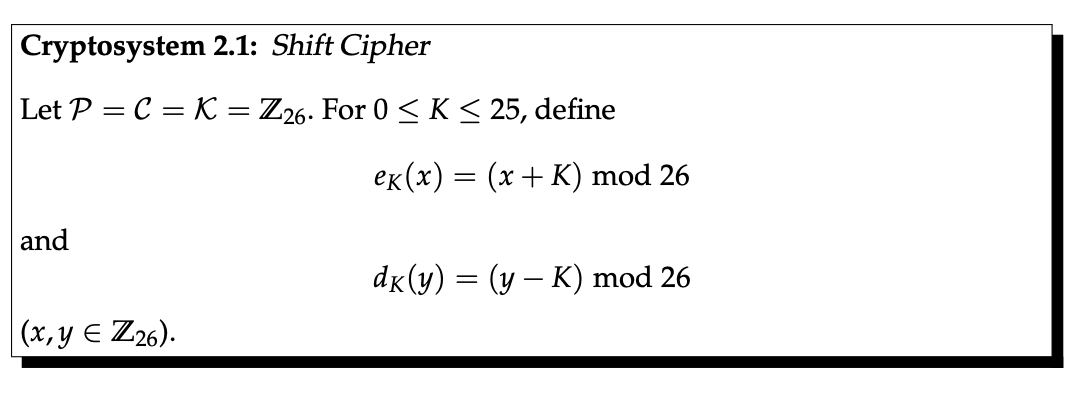
\includegraphics[scale=0.6]{cesare}
\end{center}
Il cifrario di cesare lavora quindi associando un valore numerico (solitamente da 0 a 25, siccome vi sono 26 caratteri nella lingua italiana), e shiftando l'alfabeto a destra/sinistra per $k$ valori, ove $k$ è la chiave. Il processo di decifrazione avviene shiftando $k$ valori indietro le corrispondenze.

\subsection*{Quadrato di Polibio}
\begin{center}
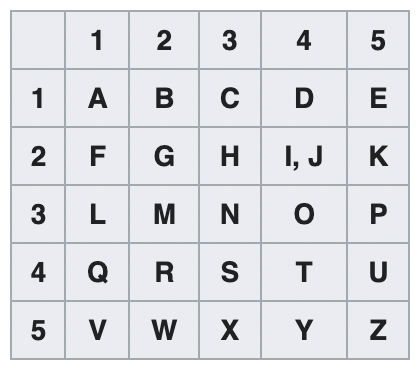
\includegraphics[scale=0.6]{polibio}
\end{center}
Il cifrario basato sul quadrato di Polibio funziona creando una matrice $n * n$, nella quale si inseriscono le lettere all'interno, per ogni corrispondenza si prende al coppia \emph{riga, colonna}.
Intuitivamente la il ciphertext è grande il doppio del plaintext, il problema principali con questo cifrario è la presenza di punti fissi.

\subsection*{Una naturale evoluzione}
La presenza di punti fissi ci porta a cercare un modo di migliorare questi cifrari, in particolare un approccio migliore è passare da espressioni 
\begin{center}
\(y = x + k \) $\rightarrow$ \(y = \alpha x + \beta \) \\
con \(\alpha \neq 0   , \beta \neq 0 \)
\end{center}
Per ricavare un valore dobbiamo facciamo 
\begin{center}$\frac{(y-\beta)}{a} = x$ 
\end{center}
E' inoltre importante che MCD($\alpha, 26)$ = 1 ovvero che $\alpha$ sia invertibile, e che $\alpha$ e 26 siano \emph{coprimi}

\subsection*{Attaco ai cifrari affini}
\emph{Come attacchiamo i cifrari affini?} Andiamo ad analizzare le frequenze\\
In italiano le lettere che compaiono di più sono E (che compare in media 11,79\%), la A (11,74\%), la I (11,28\%) etc.\\ Più il testo è lungo, più possiamo essere certi della corrispondenza (maggiore il campione, migliore l'approssimazione). Il problema del cifrario affine è quindi che data una lettera, la corrispondenza cifrata è sempre la stessa.

\subsection*{Quadrato di Vigenère}
\begin{figure} [H]
\begin{center}
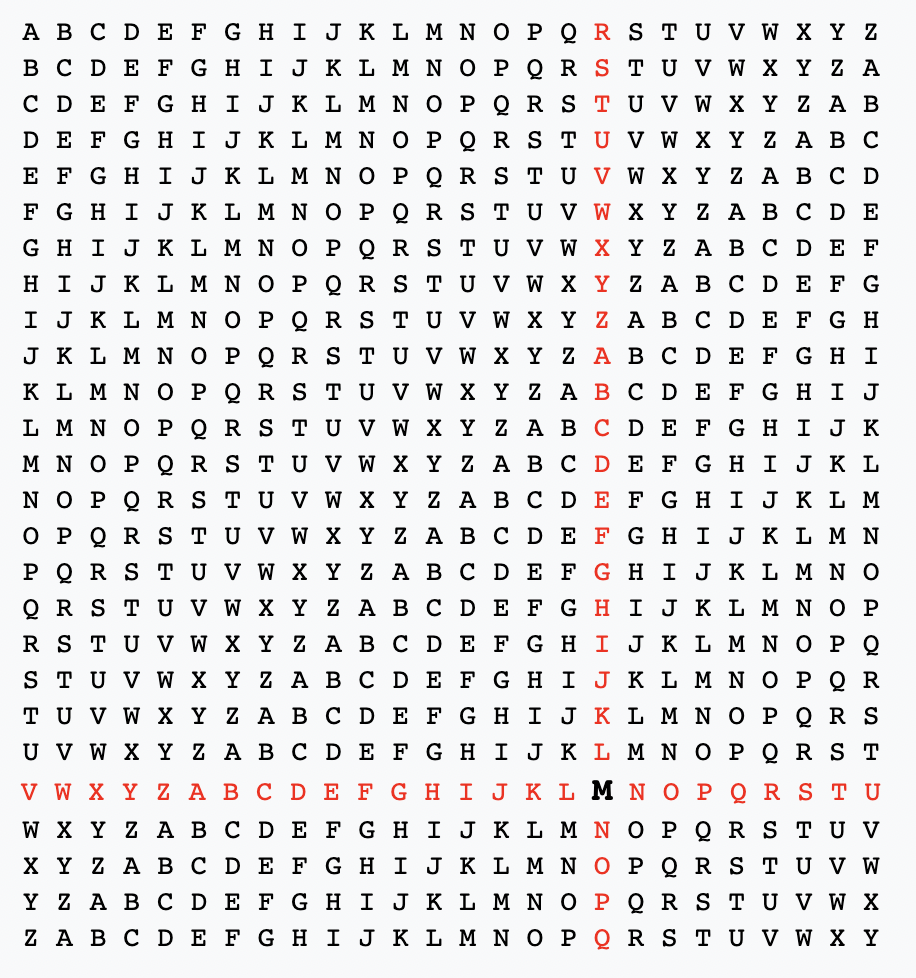
\includegraphics[scale=0.4]{vig}
\caption{codifica della lettera R con chiave V}
\end{center}
\end{figure}
Il quadrato di Vigenère lavora nel seguente modo: il mittente ed il destinatario concordano una parola, chiamata chiave. 
La chiave è ripetuta $n$ volte fino a ricavare una corrispondenza 1-1 con la lunghezza del messaggio da cifrare. \\
Per ricavare le singole lettere andiamo a ricavare la corrispondenza con colonna \begin{center}
\(Cyphertext_i = (Plaintext_i, Chiave_i)\)\\
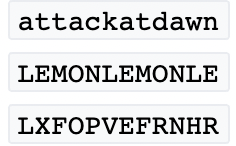
\includegraphics[scale=0.7]{chiave}
\end{center}
Come attacchiamo questo cifrario? Il metodo più famoso è il metodo di Kasiski\\
Attraverso \emph{l'analisi di Kasiski} possiamo sfruttare il fatto che alcune parole, per probabilità, vengono cifrate con le stesse lettere. Questo ci permette di trovare gruppi ripetuti nel \emph{cyphertext}.
\begin{center}
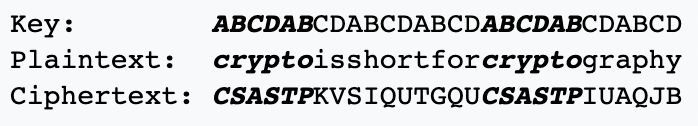
\includegraphics[scale=0.7]{freq}
\end{center}
Una volta identificati questi gruppetti, li raccogliamo e possiamo essere certi che questi sottoinsieme saranno un divisore della chiave. Possiamo quindi effettuare un'analisi di frequenza su queste, più lunga il testo, migliore sarà la precisione dell'analisi di frequenza.\\
Una variante è il cifrario di Cardano, in cui la chiave è inserita prima del crittotesto, tecnica molto vulnerabile in quanto è l'attaccante deve solo indovinare la lunghezza.

\subsection*{Playfair cipher}
Il cifrario è basato su una matrice 5x5 (essendo l'alfabeto di 26, una lettera ha una corrispondenza con un'altra, solitamente i con j) in cui vengono inserite le lettere. Si utilizza una parola come chiave e le lettere sono inserite saltando i doppioni, mettendo in testa la chiave.
\begin{center}
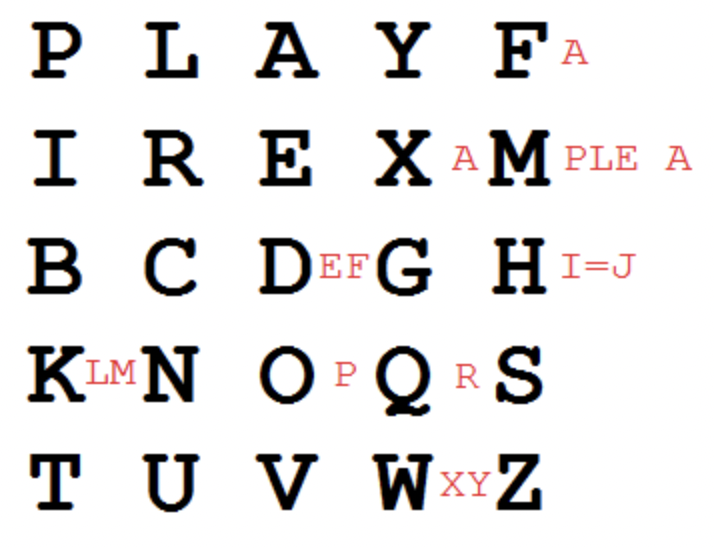
\includegraphics[scale=0.5]{playfair}
\end{center}
Il cyphertext è creato a coppia di lettere, formando un rettangolo/quadrato utilizzando i vertici opposti delle due lettere scelte. I vertici opposti rappresentano le lettere cifrate.
\begin{figure} [H]
\begin{center}
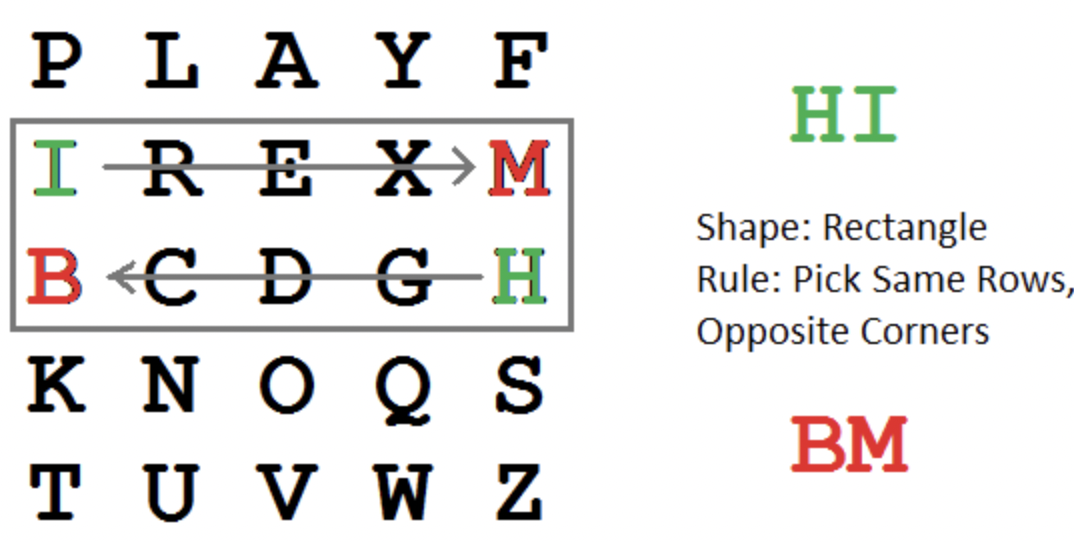
\includegraphics[scale=0.5]{playfair2}
\caption{I vertici opposti del rettangolo delle lettere HI sono BM, la codifica è BM}
\end{center}
\end{figure}

\subsection*{Hill cipher}
Viene definita una matrice \emph{k} di dimensione \emph{n * n}, le parole vengono cifrate a coppie di n (matrice 2 x 2, cifrate 2 alla volta, matrice 3 x 3, cifrate 3 alla volta).\\
Consideriamo il seguente alfabeto con corrispondenti numeri
\begin{center}
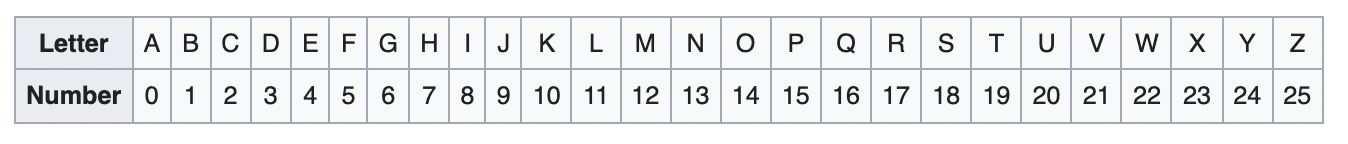
\includegraphics[scale=0.5]{hill}
\end{center}
Per codificare un messaggio, ogni blocco di $n$ lettere è moltiplicato per una matrice $n * n$ invertibile, modulandolo a 26. per decifrare il messaggio ogni blocco è moltiplicato per l'inverso della matrice utilizzata durante la fare di cifratura.
Non tutte le matrici chiavi sono ammissibili, la matrice deve esser invertibile per permettere il decifraggio da parte del destinatario. In particolare \(MCD(\Delta, 26) = 1\).\\
Consideriamo il messaggio \emph{ACT}, con chiave \emph{GYB/NQK/URP}
\begin{center}
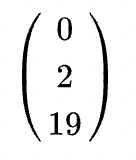
\includegraphics[scale=0.5]{2}
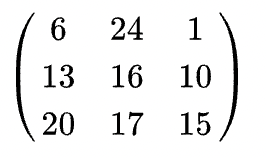
\includegraphics[scale=0.5]{1}
\end{center}
Il processo di cifratura avviene così:
\begin{center}
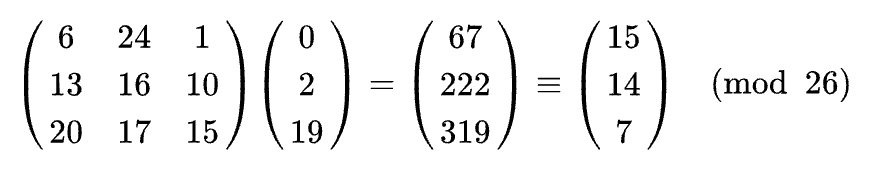
\includegraphics[scale=0.5]{3}\\
\emph{ove 15, 14, 7 corrisponde a POH}
\end{center}
E la fase di decifratura avviene intertendo la matrice iniziale modulo 26, e moltiplicandolo per il ciphetext:
\begin{center}
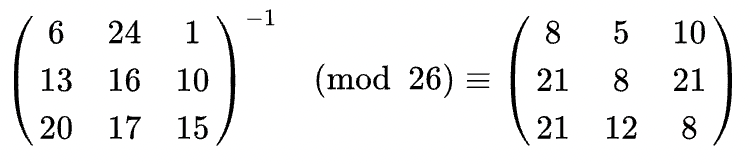
\includegraphics[scale=0.5]{4}\\
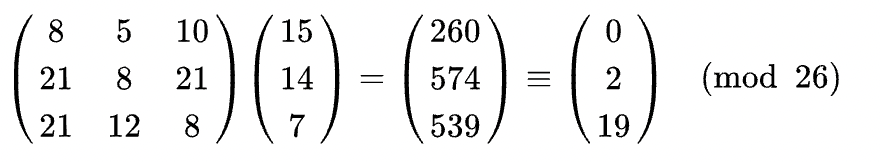
\includegraphics[scale=0.5]{5}\\
\emph{che ci restituisce nuovamente ACT}
\end{center}

\subsection*{ADFGX cipher}
Utilizzata dai generali tedeschi durante la prima guerra mondiale, viene creata una matrice 5 x 5 in cui vengono inserite le lettere arbitrariamente.
\begin{figure}[H]
\begin{subfigure}[h]{0.3\linewidth}
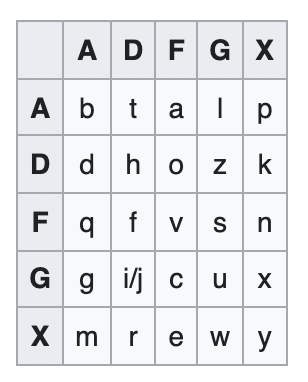
\includegraphics[width=\linewidth]{adfgx}
\end{subfigure}
\hfill
\begin{subfigure}[h]{0.6\linewidth}
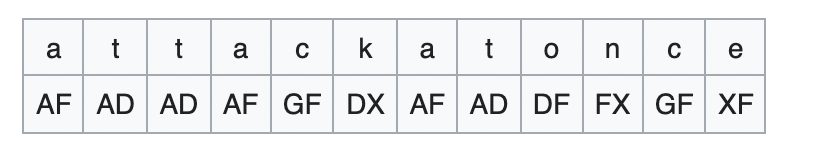
\includegraphics[width=\linewidth]{word}
\end{subfigure}%
\end{figure}
Per ricavare il crittotesto prendiamo le coppie degli indici (riga, colonna), ogni lettera quindi è data da una coppia di indici. \\Viene poi riordinato il crittotesto secondo una chiave di lunghezza k. Il crittotesto viene suddiviso in righe di k lunghezza. Una volta messe in pila di lunghezza k, le colonne vengono riordinate secondo l'ordine alfabetico delle lettere chiave.
\begin{figure}[H]
\begin{subfigure}[h]{0.2\linewidth}
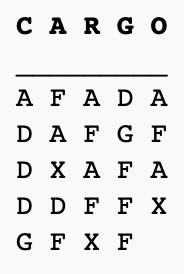
\includegraphics[width=\linewidth]{pre}
\end{subfigure}
\hfill
\begin{subfigure}[h]{0.5\linewidth}
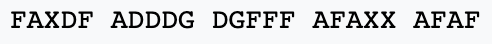
\includegraphics[width=\linewidth]{adfgx2}
\caption*{La codifica di CARGO}
\end{subfigure}
\hfill
\begin{subfigure}[h]{0.2\linewidth}
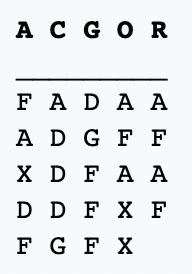
\includegraphics[width=\linewidth]{post}
\end{subfigure}%
\end{figure}
\section*{NIST / NBS}
Il NIST è un'associazione governativa americata che si occupa di emettere bandi per richiedere la creazione di cifrari per il pubblico. In questo momento i bandi aperti sono: "Post-quantum competition" del 2018 ed il "Lightweight cryptography" per sistemi leggeri.\\
Nel 1970 manda un bando per creare un cifrario simmetrico utile alle grandi aziende americane per cifrare i dati sicuri, in particolare viene sviluppato DES, un cifrario simmetrico.
\section*{Data Encryption Standard | DES}
E' un cifrario simmetrico a 16 round, basato su blocchi di 64, dotato di \emph{64 - 8 (bit di controllo) = 56} bit di chiave che produce un ciphertext di lunghezza 64. Un attacco di brute-forcing svolge al massimo $2^{56}$ tentativi, che già nel 1970 porta molti ad obbiettare.
\begin{itemize}
\item grandezza dei blocchi di plaintext: 64
\item grandezza delle chiavi: 56 (64 - 8)
\item grandezza dei ciphertext: 64
\end{itemize}
Per cifrare un messaggio con DES vi sono 3 principali sali, l'initial permutation o IP, Feistel permutation, e la final permutation FP. IP e FP non hanno valore crittografico, ma furono inseriti per facilitare il caricamento dei blocchi all'interno dei sistemi a 8 bit del 1970.
\begin{figure}[H]
\begin{subfigure}[h]{0.4\linewidth}
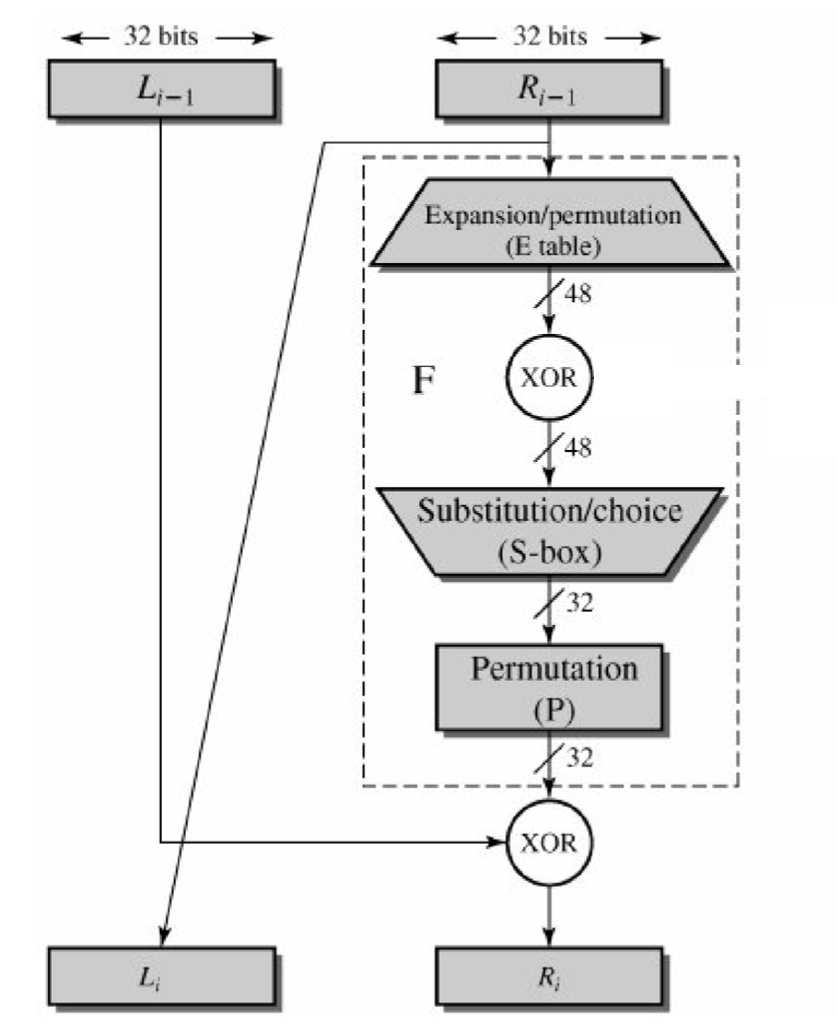
\includegraphics[width=\linewidth]{DES}
\end{subfigure}
\hfill
\begin{subfigure}[h]{0.4\linewidth}
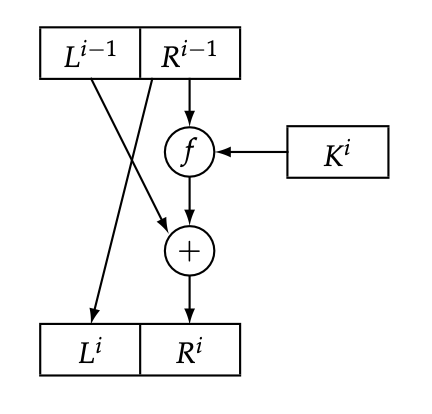
\includegraphics[width=\linewidth]{DES2}
\end{subfigure}%
\end{figure}
\subsection*{Ma dove entra in gioco la chiave?} 
La chiave è fornita alla funzione di Feistel, ed è generata per ogni dato round di cifratura
\subsection*{La funzione Feistel}
Quando parliamo di funzioni di Feistel parliamo di funzioni la cui sicurezza è acquisita effettuando \emph{n round} di permutazioni
\begin{center}
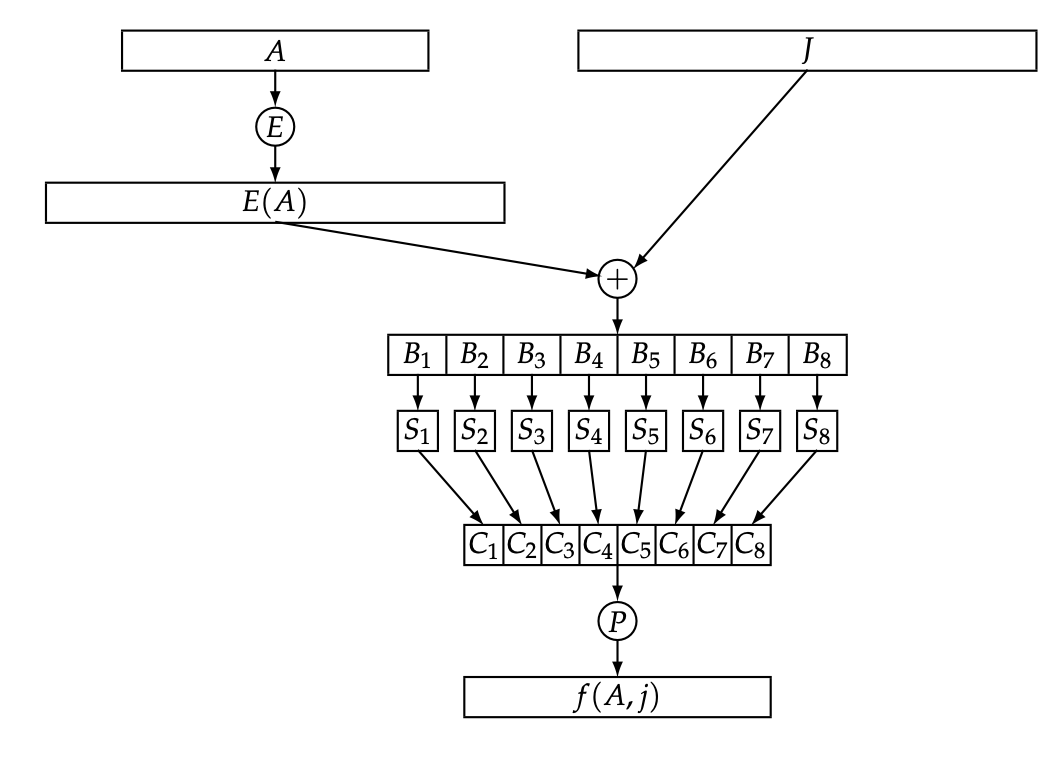
\includegraphics[scale= 0.4]{feistel}
\end{center}
\subsection*{La funzione di espansione}
La funzione \emph{E} rappresenta la permutazione di espansione, che aggiunge 16 bit ai 32 forniti in precedenza. Questi 48 bit sono utilizzati per effettuare uno XOR con \emph{J} (la chiave del round), che ci permette di ricavare 8 blocchi. Il valore in output dipende da una tabella prefissata.
Questi 8 blocchi (formati da 6 bit ciascuno) sono permutati nuovamente (all'interno di $S_k$).
\subsection*{S-Box}
Le funzioni $S_k$, rappresentate dalle S-Box, eseguono \emph{un'operazione di compressione-permutazione}: prendono in bit 6 bit ciascuno, ma restituiscono 4 bit, portando l'output a 32 bit. Questi 32 bit rappresentano l'output. $S_k$ è formato da una matrice $(4 * 16)$ sulla quale sono inseriti una permutazione dei valori tra 1 a 16 (fissa).
\begin{center}
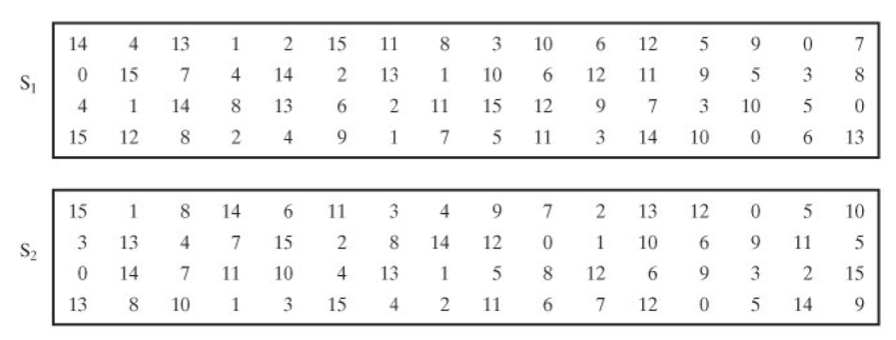
\includegraphics[scale= 0.7]{sbox}\\
\emph{un esempio di S-Box}
\end{center}
Dato una sequenza di input di bit di lunghezza 6 (l'input di ogni s-box), il primo ed l'ultimo valore sono utilizzati per indicizzare la riga, ed i 4 valori interni indicizzano la colonna.
\begin{center}
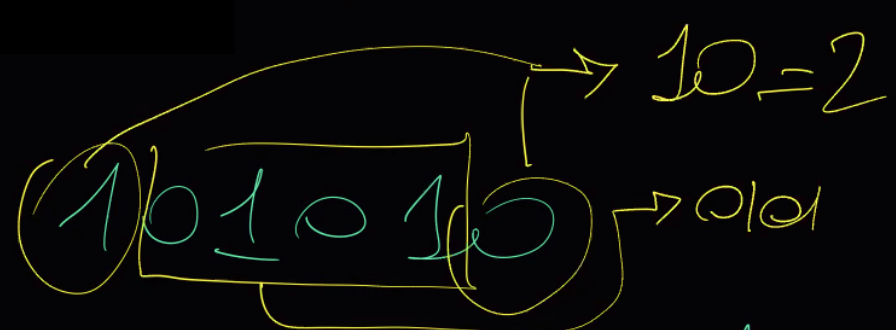
\includegraphics[scale= 0.5]{sbox1}\\
\emph{Si prende la terza e la sesta perché il binario 00 è la prima colonna, noi contiamo da 0}
\end{center}
Il valore ricavato incrociando riga e colonna codificato in binario rappresenta l'output della S-Box.
Questo è possibile perché nella matrice vi sono solo valori tra 0 e 15, che sono codificabili in binario su 4 valori.
\begin{center}
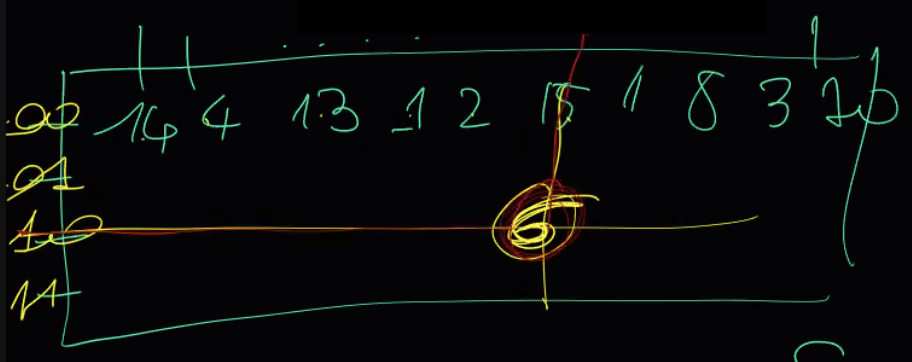
\includegraphics[scale= 0.5]{sbox2}\\
\emph{il valore di output di questa S-box sarà $0110_2$ = 6$_{(10)}$}
\end{center}
\subsection*{La chiave $K_i$}
\begin{center}
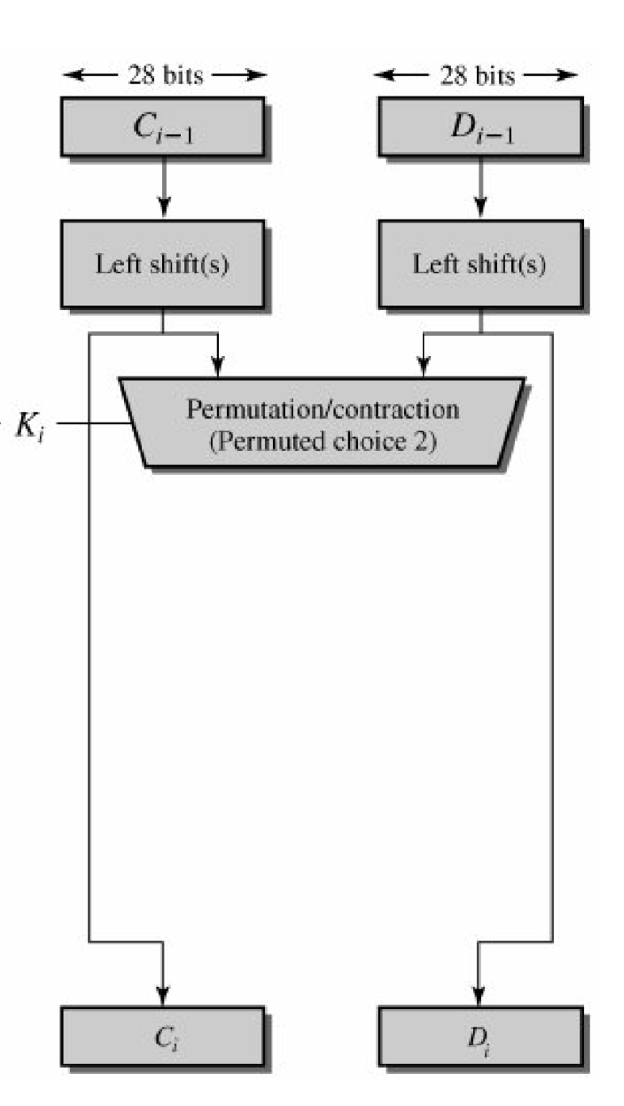
\includegraphics[scale= 0.6]{k1}
\end{center}
La chiave $K_i$ è formata da 64 bit, dalla quale vengono rimossi 8 bit di parità. Sui bit rimanenti è effettuata una permutazione. I 56 bit dopo la permutazione sono suddivisi in 2 blocchi da 28, chiamati rispettivamente $C_0$ e $D_0$. Questi sono shiftati a sinistra, ed il loro valore dipende dal numero di round.\begin{center}
$C_i$ = LS($C_{i-1}$)\\
$D_i$ = LS($D_{i-1}$)
\end{center}
Il valori shiftati vengono utilizzati come input per una permutazione/contrazione, passando da 56 a 48. L'output di questa permucontrazione rappresenta la chiave, e gli input della prossima $C_i$  e $D_i$.\\
\begin{center}
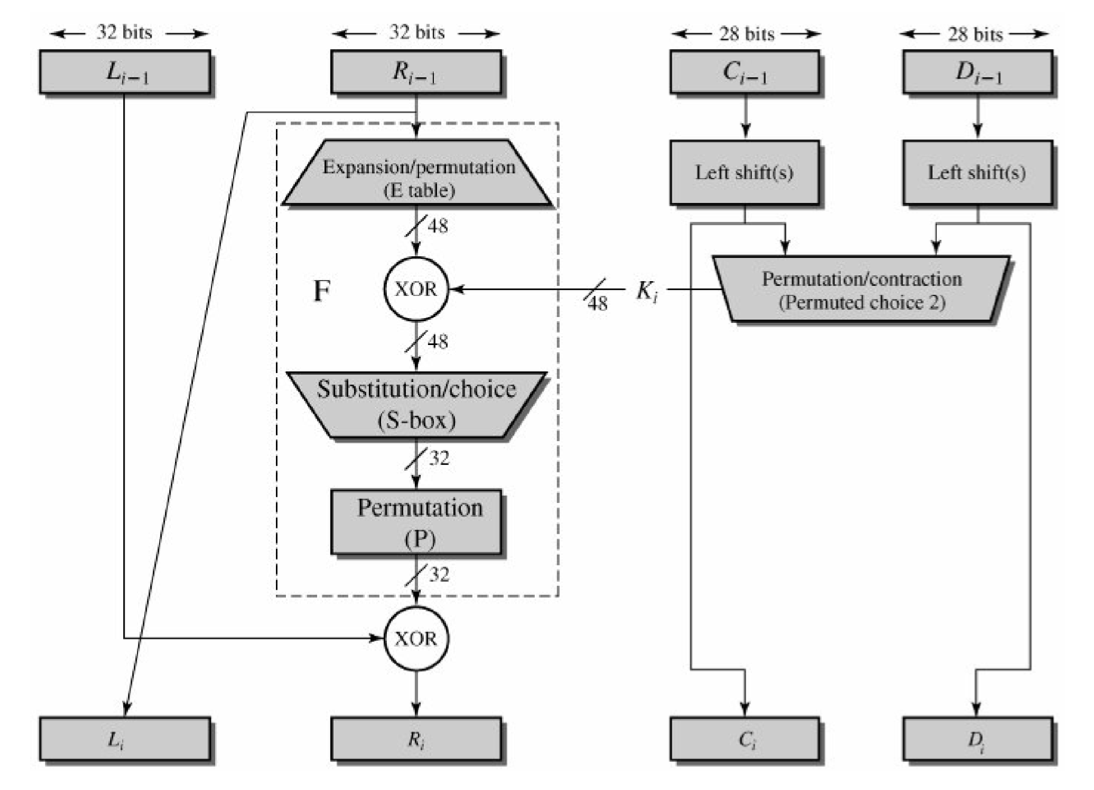
\includegraphics[scale= 0.5]{des3}\\
\emph{Overview di DES}
\end{center}
Vi sono dei vincoli riguardo a DES, per esempio:\\
E' importante che dato un S-Box, l'output di tale S-Box non possa in qualsiasi modo approssimabile.

\long\def\comment#1{
\section*{S-DES | Simplified DES}
Andiamo ora a vedere una versione semplificata di DES, con le seguenti caratteristiche:
\begin{itemize}
\item \(plaintext = 12 bits \)
\item \(L_i = 6 bits\)
\item \(R_i = 6 bits\)
\item \(k = 9 bits\)
\end{itemize}
Il numero di round è diminuito, in particolare 3 (II, III, IV), tratteremo quindi:\\ \(L_1, R_1  \rightarrow L_2, R_2 = I° $ $  round\)\\ \(L_2, R_2  \rightarrow L_3, R_3 = II°  $ $round\)\\ \(L_3, R_3  \rightarrow L_4, R_4 = III° $ $ round\)
\subsection*{La funzione di Feistel semplificata:}
\(R_{(i-1)}\) (6 bits) è passato in espansione (8 bits), e fatta passata in XOR con la chiave (8 bits) (che perde un bit), per poi essere inserita come input (di 4 bits) in 2 S-Box di compressione (matrici 2 * 8).\\
L'output delle S-boxes sono di 3 bits ciascuna, il risultato è \(f(R_{i-1}, k_i\)).\\\\
\emph{La funzione di espansione E(x):}\\
La funzione di espansione ripete dei bit dell'input. In particolare dato un input:\begin{center}
(1-2-3-4-5-6) (6 bits), l'output sarà (1-2-4-3-4-3-5-6) (8 bits) \\in cui k rappresenta la posizione \(k_i\)\\
\end{center}
\emph{Le S-Box semplificate sono:}
\begin{center}
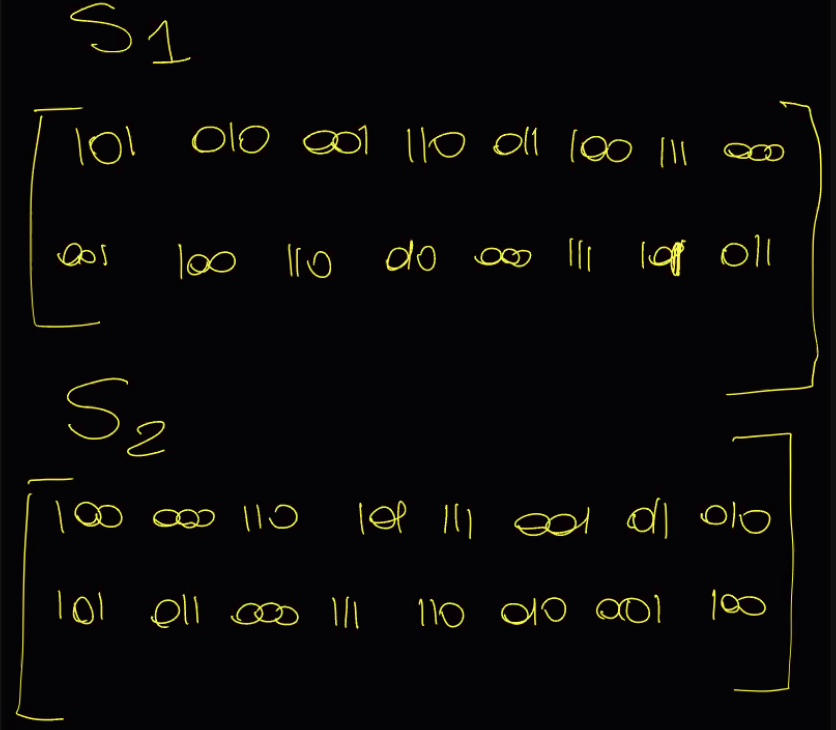
\includegraphics[scale= 0.5]{ssbox}\\
\end{center}
Per ricavare il valore di output è ricavato prendendo: il 1° bit per la riga, e gli altri 3 per la colonna\\
\emph{La compressione della chiave:}\\
La chiave è ricavata copiando la chiave a partire dalla posizione 2, ricopiando dall'inizio quando necessario.\\
\(k = 001001101\)\\
\(k_2 = 010011010\)\\
}

\section*{Attacco a DES | Crittoanalisi differenziale}
L'attacco a DES è un attacco chiamato di analisi differenziale, è un attacco deterministico se il numero di round e $\leq 3$ e diventa probabilistico dai 4 in su dovuta alla presenza di round di crittografia (round di DES). 



\subsection*{Doppio DES e triplo DES}
Doppio DES e triplo DES sono tecniche di cifratura direttamente derivate da DES, sappiamo che DES utilizza una chiave di 56 bit per cifrare un qualsiasi plaintext, per rafforzare ulteriormente l'algoritmo è stato pensato di raddoppiare le operazioni di cifratura applicando DES più volte.\\

Rispettivamente doppio DES utilizza una chiave da 112 bits, e triplo DES una chiave da 168 bits.
L'efficacia di applicazione di questi algoritmi dipende strettamente dalla scelta della chiave, in particolare se la chiave scelta è la medesima, ovvero $k_1 == k_2$, la sicurezza fornita non è di $2n$ la lunghezza della chiave, ma di $n+1$. In particolare attraverso un attacco \emph{"meet in the middle"} un attaccante può ricavare la coppia id chiavi in $2^{n+1}$ passi, piuttosto che $2^{2n}$.\\

Per ovviare a questo problema, quindi, sono state definite una serie di linee guida per la selezione delle chiavi, in particolare:
\begin{itemize}
\item Le 3 chiavi sono indipendenti, chiamato anche 3TDEA, è l'approccio migliore, che fornisce il grado di sicurezza maggiore, ovvero $3 \times 56 = 168$ bit di chiave.
\item Le chiavi $k_1$ e $k_2$ sono indipendenti, e la chiave $k_3 = k_1$, chiamato anche 2TDEA, fornisce una chiave id lunghezza inferiore, ed è un compromesso accettabile. Il NIST ha già deprecato questa opzione
\item Le chiavi $k_1, k_2, k_3$ sono identiche, come abbiamo detto in precedenza, l'adozione di questo approccio è fortemente scoraggiato in quanto non fornisce granché sicurezza aggiuntiva rispetto al DES tradizionale.
\end{itemize}

Consideriamo un ciphertext cifrato con 2 round di DES, prima con una chiave $k_1$ e poi con una chiave $k_2$. Lo sforzo computazionale per decryptare il ciphertext richiederebbe $2^{56} + 2^{56}$ tentativi ovvero $2^{57}$, rispettivamente per ogni round.
\begin{center}
$C= E(k_2;E(k_1;p))$
\end{center}
\emph{Esiste una chiave $k_3$ che possa passare direttamente da plaintext a ciphertext?}\\
 - La risposta è no\\
 Il problema con questa implementazione è che le chiavi da mantenere diventano 2: $k_1, k_2$. Per arginare questo problema possiamo trasformare la funzione di encryption in:
 \begin{center}
 $C = E_{k_1}(D_{k_2}(E_{k_1}(plaintext)))$\\
 \emph{Ove $E$ è l'operazione di encryption, mentre $D$ è l'operazione di decryption}
 \end{center}
 Questa tecnica è chiamata \emph{Triple-DES o 3-DES} ed è il meccanismo alla base dei pagamenti elettronici. La decryption è effettuata con la chiave $k_2$, che però è diversa dalla chiave $k_1$, aggiungendo ulteriormente entropia.\\Se $k_1 == k_2$ l'operazione di encryption è svolta una sola volta (single DES), che ci permette di comunicare anche con dispositivi datati che non supportano l'encryption basato su più chiavi.
 


\section*{Le modalità di cifratura ECB, CBC, CFB, OFB, CTR}
Vediamo le modalità di utilizzo dei cifrari a blocchi, applicabili su qualsiasi cifrario a blocchi:
\subsection*{ECB, o "electronic codebook mode":}
ECB è applicato dividendo il plaintext in blocchi di equa grandezza, che vengono poi codificati in cyphertext attraverso una cifrario a scelta. La dimensione del blocco è dipendente dal cifrario scelto\\
ECB è ideale quando la quantità di dati da codificare è bassa, se per esempio si vuole traasmettere una chiave DES, ECB è ideale.\\
Dato: \begin{center}
$P = [p_1, ..., p_n]$ l'insieme delle porzioni di grandezza n\\
$C = [c_1, ..., c_n]$ l'insieme dei ciphertext di grandezza n
\end{center}
attraverso la funzione
\begin{center}$f(P_i; DES) = C_i$ 
\end{center}
Codifichiamo un plaintext in ciphertext. Per ricavare il plaintext utilizziamo la funzione di decryption su ogni blocco di ciphertext.
\begin{center}
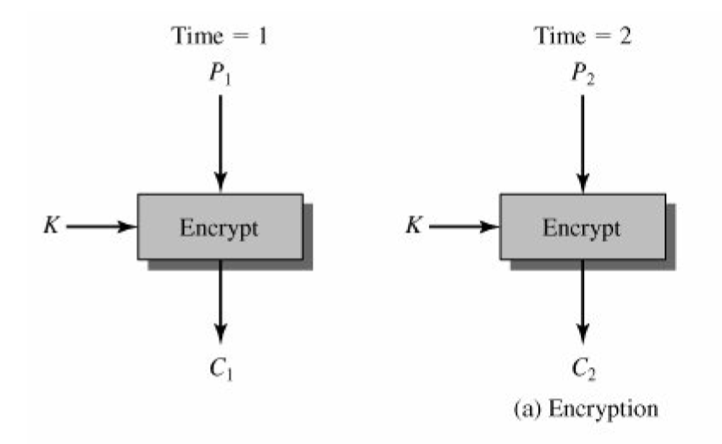
\includegraphics[scale= 0.7]{ecb}
\end{center}
Il problema con ECB è che se più blocchi di plaintext sono uguali, il ciphertext prodotto è uguale. Questo permette su messaggi molto lunghi di essere attaccati attraverso una crittoanalisi di frequenza
\subsection*{CBC, o "cipher block chaining mode":}
Per mitigare le falle di sicurezza di ECB, vogliamo introdurre un meccanismo per produrre ciphertext differenti per plaintext diversi. \\
Con CBC introduciamo un round di XOR con una chiave IV (Initialization vector)(pubblica o privata) prima della fase di encryption, per offuscare ulteriormente il plaintext. IV è sostituito dal ciphertext del round $P_i-1$ dalla fase 2 in poi.
\begin{center}
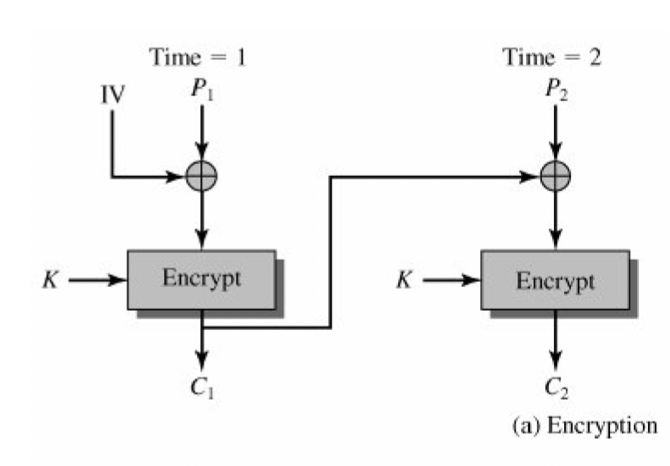
\includegraphics[scale= 0.7]{cbc}
\end{center}
In parole povere introduciamo una chiave \emph{IV} da applicare in XOR con la prima fase di encryption. Dalla seconda fase in poi l'IV è sostituito con il ciphertext del round $P_i-1$.

\subsubsection*{The underlying problem:}
Il problema con queste modalità è che l'operazione di cifratura avviene su singoli blocchi, piuttosto che su singoli caratteri. Sarebbe comodo poter trasmettere singoli blocchi cifrati alla volta

\subsection*{CFB, o "cipher feedback mode":}
In questo schema di encryption, il vettore di inizializzazione è encryptato con la chiave $k$. $n = 8$ bits dell'output sono utilizzati come input per un'operazione di XOR con il plaintext, che è stato in precedenza suddiviso in blocchi da 8 bits. L'output è inserito in coda al vettore di inizializzazione prossimo, shiftando l'IV precedente.
\begin{center}
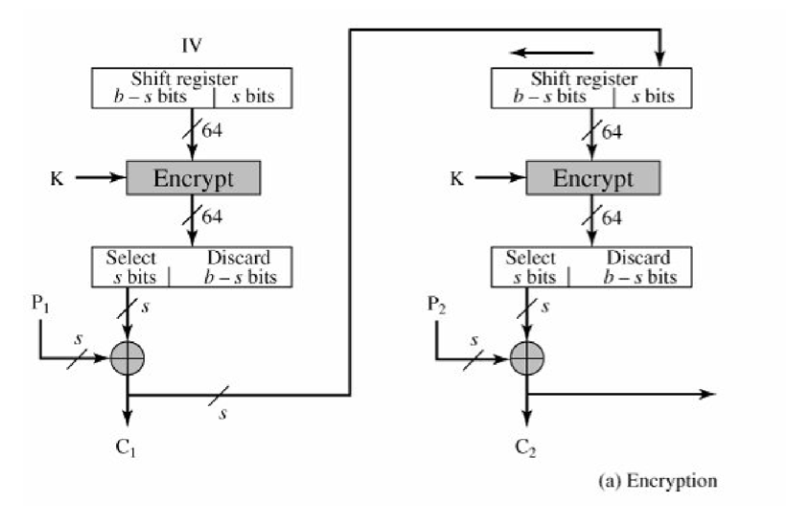
\includegraphics[scale= 0.7]{cfb}\\
\emph{da notare che l'output di encrypt sono 64 bit. \\si prende il primo blocco e quindi un char (8bits)}
\end{center}
In questa modalità la grandezza dei blocchi del plaintext è $s$ (di Select s-bits). \\Se $s = 1 char (8 bits)$, i blocchi del plaintext sono grandi $s$. \\
Il problema con questa modalità è che se compare un errore di trasmissione esso si propaga, fintanto che il blocco corrotto non venga espulso dall'IV.
\subsection*{OFB, o "output feedback mode":}
Questo schema di encryption è molto simile a CFB, ma che risolve il problema di propagazione di errore di trasmissione. Il feedback, che in CFB proveniva dopo allo XOR con il plaintext, viene piuttosto estratto in locale, prima dello XOR.
\begin{center}
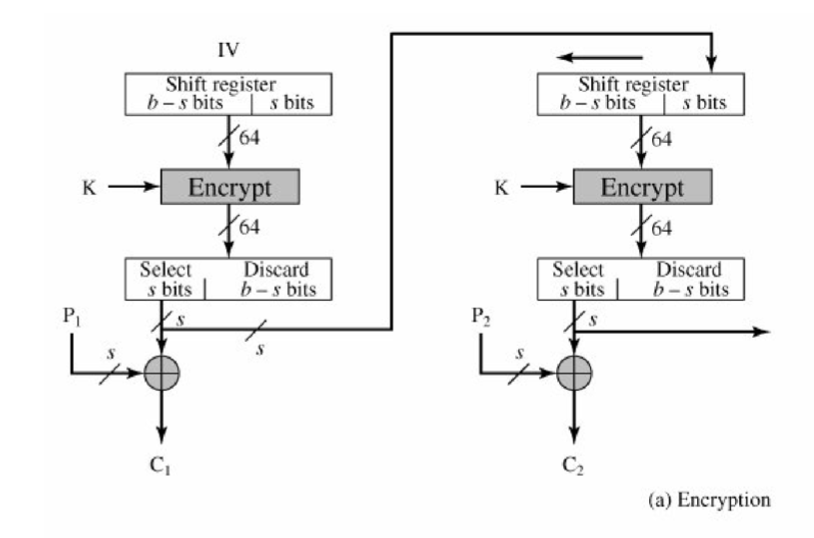
\includegraphics[scale= 0.7]{ofb}
\end{center}
Il problema con questa modalità è che le operazioni avvengono necessariamente sequenzialmente, piuttosto che in parallelo. 
\subsection*{CTR, o "counter mode":}
Viene introdotto un counter che ha grandezza uguale al plaintext (che tuttavia deve essere necessariamente diverso rispetto ad ogni plaintext che si vuole encryptare). Le due parti devono concordarsi sul valore del counter iniziale, ma siccome il valore del counter è deterministico ed indipendente l'uno dall'altro, possiamo parallelizzare le operazioni di encryption.
\begin{center}
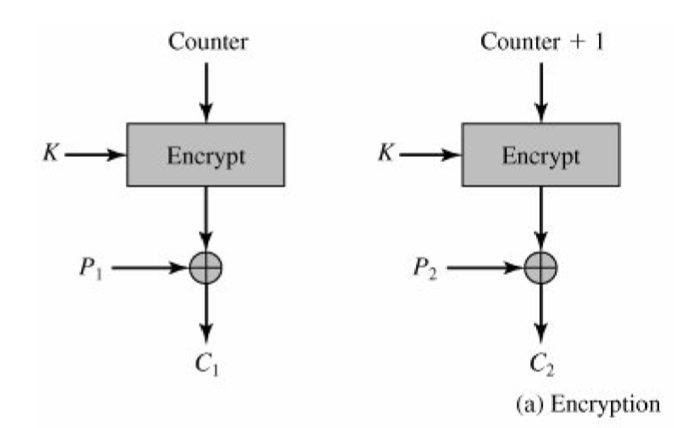
\includegraphics[scale= 0.7]{ctr}\\
\end{center}
\subsection*{XTS, o XEX-based tweaked-codebook mode with ciphertext stealing:}
Modalità di cifratura applicata su dischi. \\
%Non possiamo utilizzare $2^{256}$ perché 256 non è un numero primo. 
E' basato su un polinomio irriducibile di grado 8 sul campo di Galois che ha grado massimo 7, ovvero\begin{center}
 $GF(2^8)$ : $ax^7+bx^6+cx^5+dx^4+ex^3+fx^2+gx^1+ h$ (range dei byte)
 \end{center}
Il polinomio \begin{center}$m(x) = ax^8+bx^7+cx^6+dx^5+ex^4+fx^3+gx^2+ hx^1 + i$ \end{center}funge da modulo. Il grado è 8 perché quando andiamo ad effettuare il modulo, il risultato sarà sicuramente di grado $<$ $8$ che rientra ancora nel campo di Galois.\\ I termini $a,b,...,i$ appartengono a $Z_2$ (0, 1)\\\\
Consideriamo $(x^7+1)x^7 = x^{14} + x^7$, come possiamo vedere il risultato sfora oltre il range dei byte gestiti.
Come nel cifrario di cesare effettuiamo un modulo, rispetto ad un polinomio $m(x)$ di grado 8
\begin{center}
$x^{14} + x^7 mod(m(x))$
\end{center}
\emph{Ma quale m(x) dobbiamo utilizzare?} \\Selezioniamo un $m(x)$ di grado 8 irriducibile (sono circa 30), ad esempio: \begin{center}
$m(x) = x^8 + x^4 + x^3 +x+1$
\end{center}
Questo polinomio irriducibile è quello che è stato selezionato per AES.\\
Consideriamo $m(x)$, la sua scomposizione è: \\$m(x) * q(x) + r(x)$, e sul campo di Galois la rappresentazione di $m(x)$ è $r(x)$ \\\\
\emph{Cosa succede se ad AES applichiamo un polinomio $m'(x)$, ovvero un altro polinomio di grado 8 irriducibile ?}\\
In questo caso otterremmo un $r'(x)$, ovvero una rappresentazione diversa di $m(x)$
 
\section*{AES | Rijndael cipher}
Nel 1997 il NIST indice un nuovo contest per determinare un successore a DES, che verrà chiamato AES. Questo è fatto perché DES, avendo una chiave di 56-bit, era diventato vulnerabile ad attacchi brute force.\\
I 5 cifrari concorrenti arrivati alla finale sono: \emph{Rijndael, Serpent, Twofish, RC6, MARS}, Rijndael è selezionato nel 2001 in base a test di performance, efficienza su hardware datato, e supporto a chiavi di grandezza superiore e variabile.\\\\
In particolare AES:
\begin{itemize}
\item il plaintext ha blocchi di grandezza fissa 128 bits
\item la chiave a grandezza variabile: 128 (10 round), 192 (12 round) e 256 (14 round) bits
\item il ciphertext ha grandezza 128 bits
\end{itemize}
\begin{center}
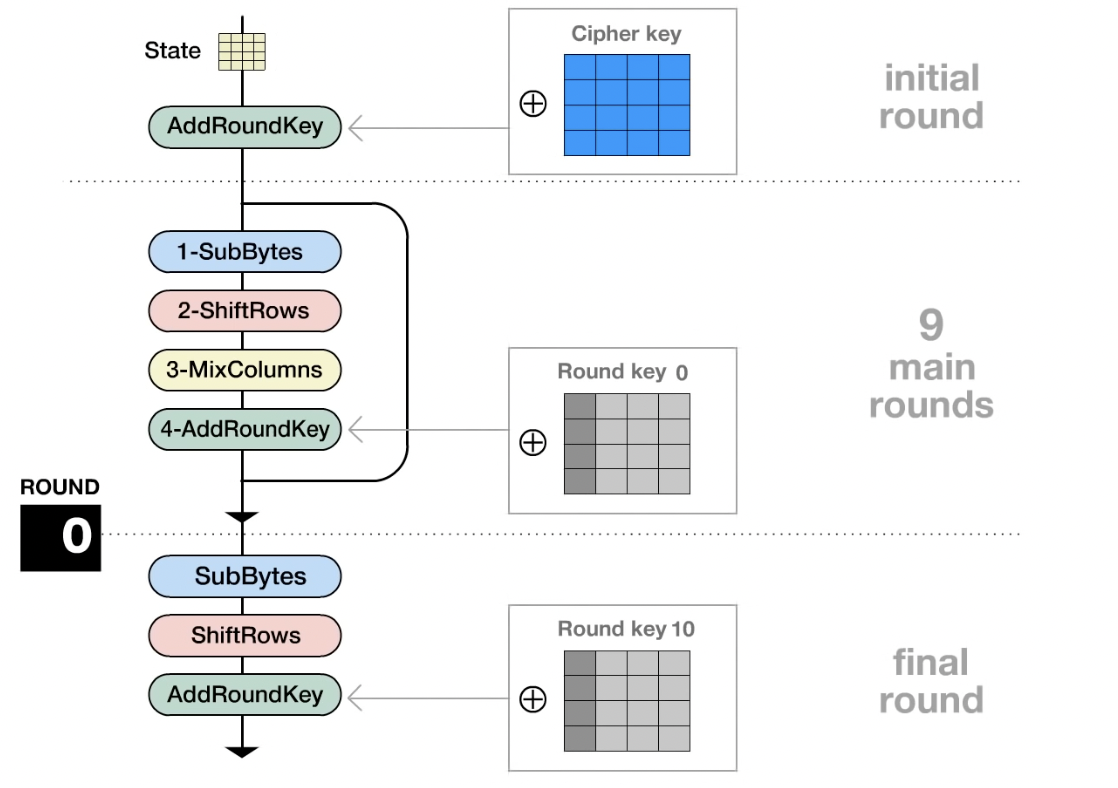
\includegraphics[scale= 0.4]{AES}
\end{center}
\subsection*{Add-round key}
E' l'operazione di "whitening" e ha l'obiettivo di neutralizzare il potenziale attacco basato su plaintext particolari (tutti 0, tutti 1 etc), consiste in un'operazione di XOR con la chiave colonna per colonna.
\subsection*{$Round_n$}
Le operazioni all'interno del $round_n$ sono svolte 9 volte e sono:
\begin{itemize}
\item Substitute bytes: corrisponde alle s-box in DES. in base ai valori presenti nello stato, vengono presi i valori all'interno di una matrice. Le s-box in AES sono di dimensione $16 * 16$\\
\emph{Ma come vengono calcolati i valori da inserire all'interno dell's-box?}
\begin{center}
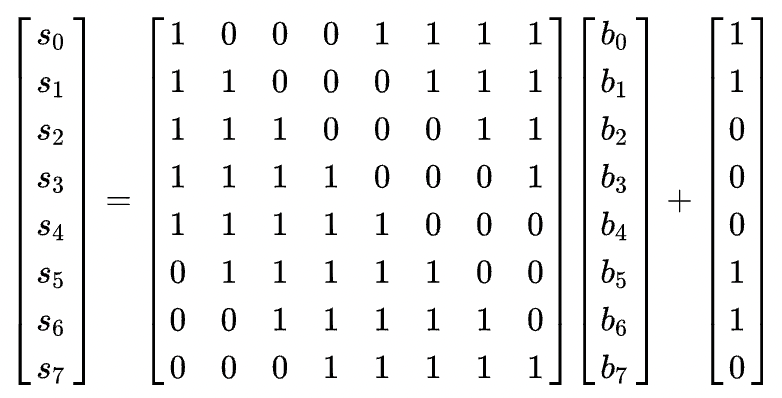
\includegraphics[scale= 0.4]{aesbox}
\end{center}
- Calcoliamo l'inverso moltiplicativo del valore $yx$ (ove. $riga = y$ e $colonna = x$) sul campo di Galois $GF(2^8)$\\
- Il byte risultante lo moltiplico per la matrice M\\
La matrice M è una matrice che è composta da n righe, costruite shiftando progressivamente verso destra il valore la seguente sequenza di bit: \begin{center}
1000 1111\\
1100 0111\\
...\\
fino a raggiungere\\
0001 1111
\end{center}
- Lo sommo per un valore costante C di valore 63\\
Il valore risultate è il valore da inserire all'interno della s-box in riga $y$ e colonna $x$.\\\\
Ricaviamo il valore a partire da 95:\\
- L'inverso moltiplicativo di 95  è $({95})^-1 = 8A$ \\
- Moltiplico l'inverso moltiplicativo per la matrice M (prodotto riga per colonna con la codifica in binario di $8A$)\\
- Faccio la somma con il valore 63 codificato in binario (11000110)\\
Il valore ricavato in riga 9, colonna 5 è 2A
\begin{center}
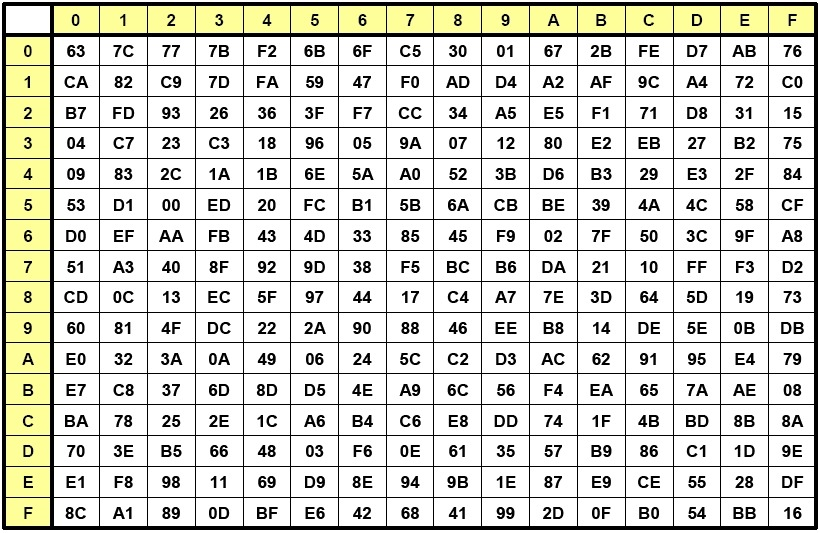
\includegraphics[scale= 0.3]{sbox3}
\end{center}
\item Shift rows: la prima riga viene lasciata invariata, la seconda viene shiftata di un byte a sinistra, e la terza viene shiftata di due byte a sinistra e la quarta di 3 byte a sinistra.
\item Mix columns: viene moltiplicata una colonna degli stati per una matrice nota, una colonna alla volta.
\end{itemize}


\subsection*{AES-XTS: meccanismo di cifratura nel disco}
AES XTS è la modalità di cifratura adottata per la cifratura dei dati su disco, in particolare adottata per evitare che due dati con lo stesso dato abbiamo la stessa cifratura (che ci espone ad attacchi di tipo analisi di frequenza). Consideriamo lo schema generale della modalità:
\begin{center}
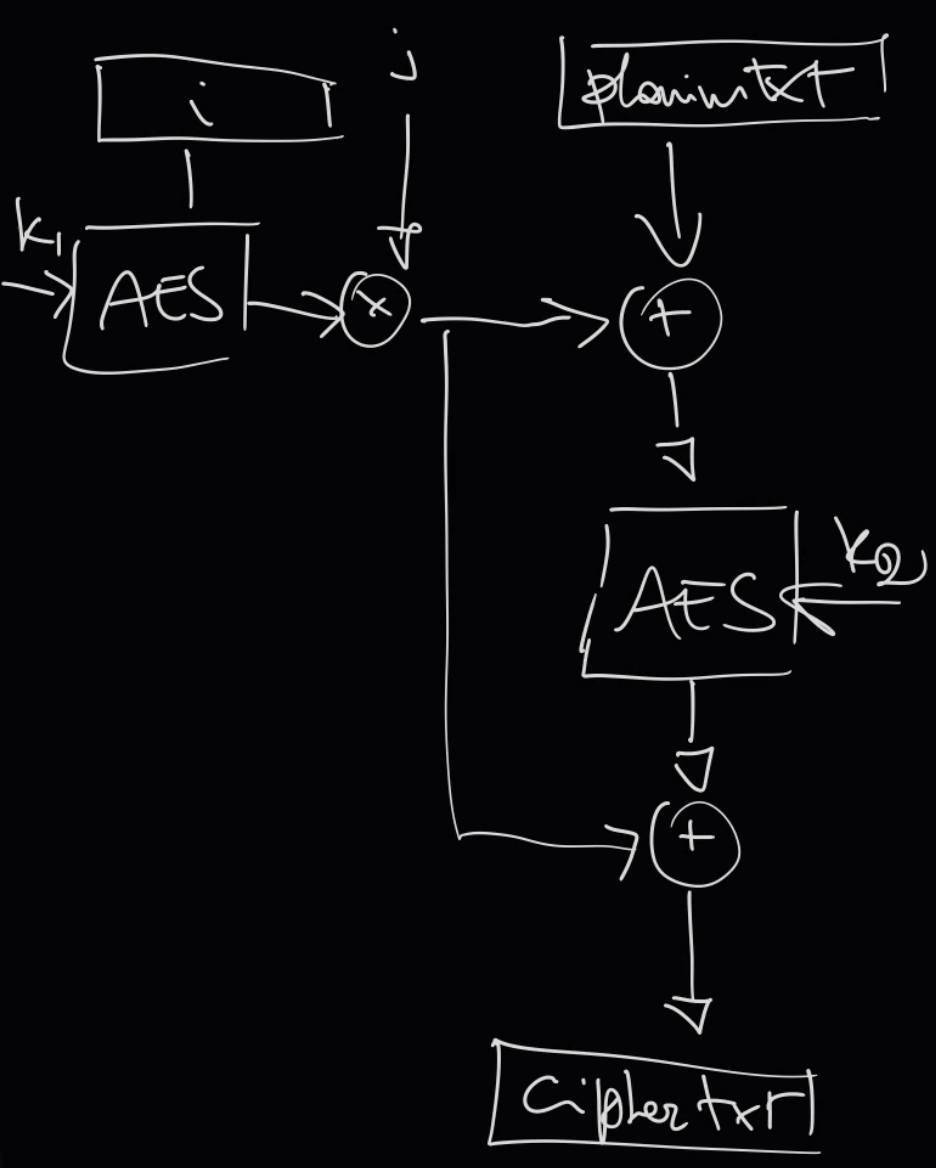
\includegraphics[scale= 0.4]{aesxts}
\end{center}
- AES $k_1$ e $k_2$ sono le due porzioni di chiavi di chiave AES applicate. $k_1$ e $k_2$ hanno dimensione 128, se la chiave AES ha 256 di dimensione. (Sono come il left and right)\\\\
- $i$ e $j$ sono rispettivamente il settore e la traccia del disco e hanno grandezza 128 bit. L'operazione che si svolge con $j$ è quella di prodotto (settore cifrato * traccia (non cifrata)). \\L'output è un polinomio in campo $GF(2^{128})$ con coefficienti su $Z_2$, con modulo $m(x) = x^{128}+x^7+x^2+x+1$\\
- Questo output è utilizzato per fare lo XOR con il plaintext, svolgendo un'operazione di whitening, prima di passare all'operazione di $AES_{k_2}$, passando per un whitening ulteriore abbiamo l'output.\\\\

\subsection*{Padding per l'ultimo blocco}
E' talvolta possibile che l'ultimo blocco non sia perfettamente di grandezza 128, 192, 256, in questo caso viene svolta un'operazione speciale per generare il padding. \\
Sia un plaintext diviso in blocchi $P_1, ... P_{m-1}, P_m$ con $P_m$ incompleto, in AES-XTS i blocchi  $P_1, ..., P_{m-2}$ sono gestiti normalmente, mentre i blocchi $P_{m-1}$ e $P_m$ sono gestiti in maniera speciale. In particolare:
\begin{itemize}
\item Il blocco $P_{m-1}$ è passato in AES-XTS, generando 
\begin{center}
$AES-XTS(P_{m-1}) = (C_{m}, CP)$
\end{center}
\item il blocco $P_{m}$ è incompleto, ed è complementato da un padding, in particolare n digits dal ciphertext $CP$ del blocco precedente.
\begin{center}
$AES-XTS(P_m, CP_n) = C_{m-1}$
\end{center}\end{itemize}
\begin{figure}[H]
\begin{subfigure}[h]{0.4\linewidth}
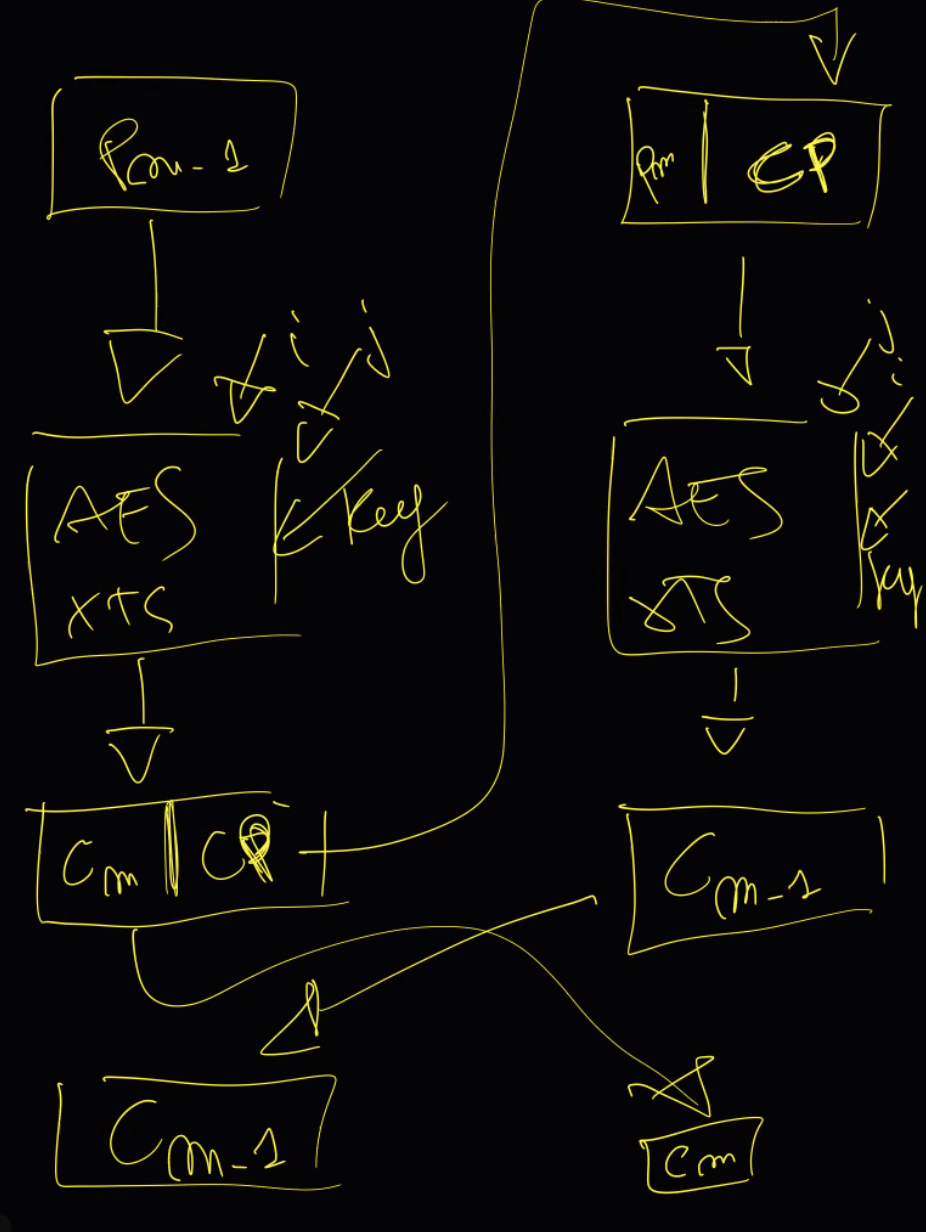
\includegraphics[width=\linewidth]{cpo}
\caption*{fase di encryption}
\end{subfigure}
\hfill
\begin{subfigure}[h]{0.4\linewidth}
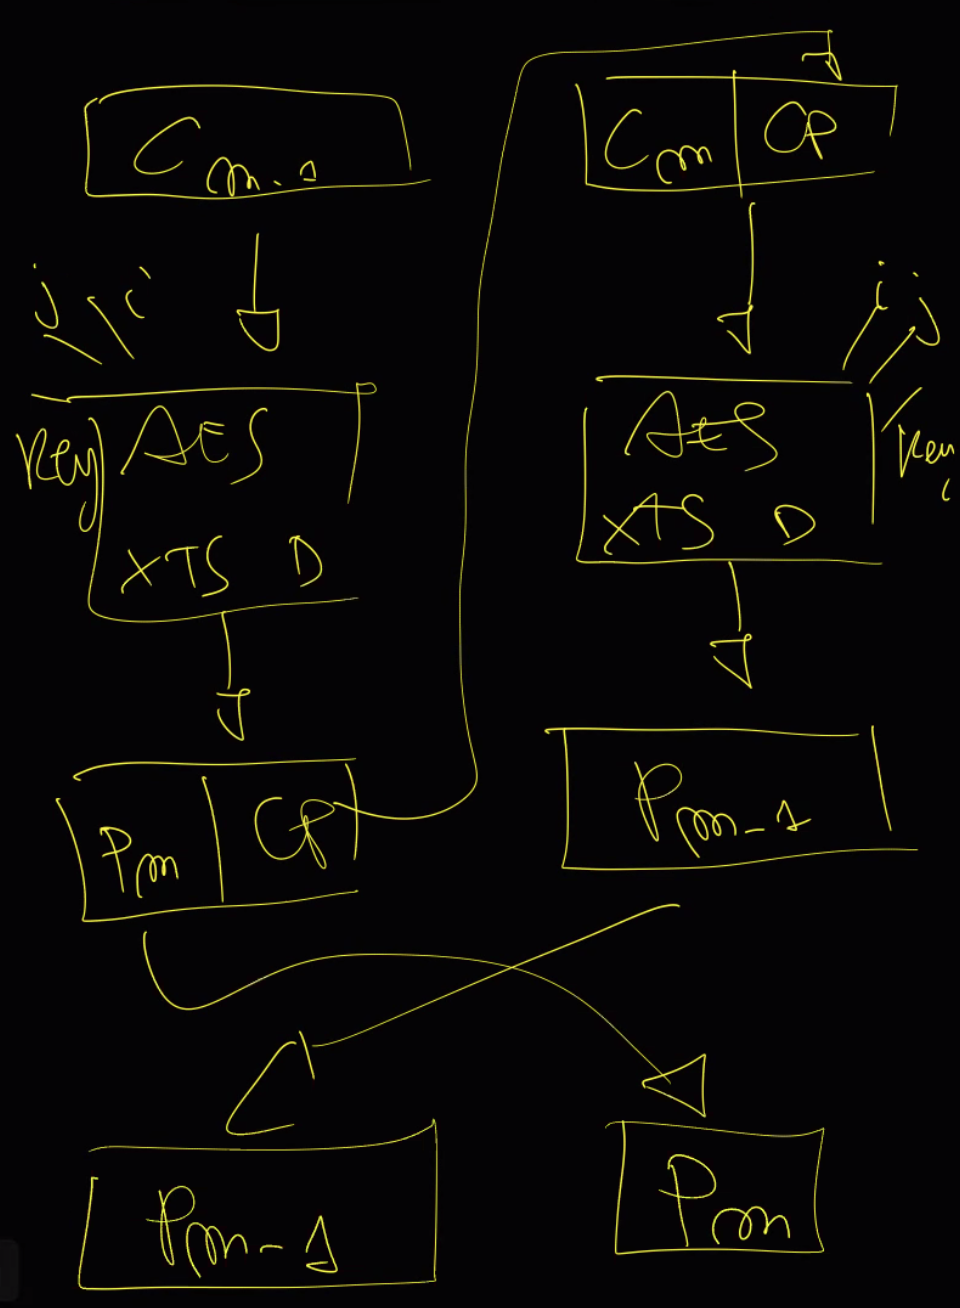
\includegraphics[width=\linewidth]{cpo-1}
\caption*{fase di decryption}
\end{subfigure}%
\end{figure}
La fase di decryption funziona al contrario (figure 2)


\section*{Attacking AES (6 rounds)}
\subsection*{Proprietà del $\Delta$ set}
Consideriamo un set di 256 plaintexts, riempiti tutti di 0. Se selezioniamo una cella all'interno dei 256 stati, e le permettiamo di assumere tutti i valori possibili in un range di un byte, ovvero da $00$ a $ff$ questa viene chiamata proprietà $\Delta$ set. $\Delta - SET$ e rappresenta l'insieme dei valori da 0 e 256. Una proprietà particolare del $\Delta - SET$ è la proprietà della \emph{somma zero}, che ci garantisce che la somma delle celle in un  $\Delta - SET$ sarà uguale a 0.\\

La proprietà di  $\Delta - SET$ è garantita fino al secondo round, ma viene persa al terzo round.
In particolare selezioniamo un index che può assumere tutti questi valori una cella attiva. 
\begin{center}
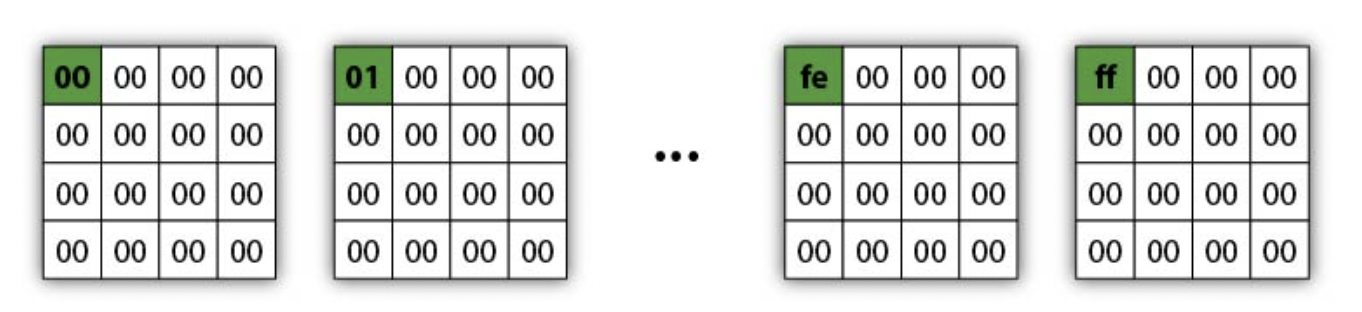
\includegraphics[scale= 0.4]{deltaset}
\end{center}
Consideriamo uno stato iniziale con proprietà $\Delta$ set, quando questa viene cifrata utilizzando AES passa all'interno di una serie di trasformazioni, in particolare:
\begin{center}
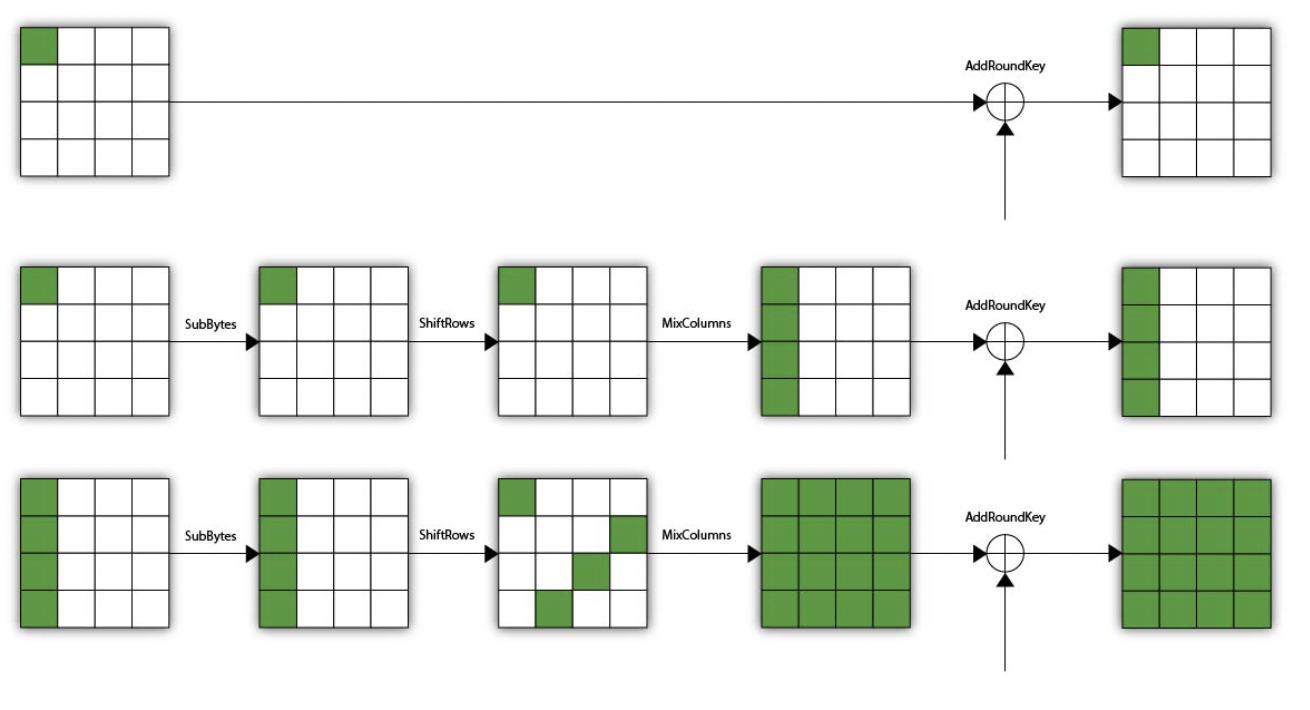
\includegraphics[scale= 0.4]{deltaset2}
\end{center}
Come possiamo vedere la proprietà di $\Delta$ set è mantenuta sia all'operazione di preambolo $AddRoundKey$, che dopo tutto il primo round, fino all'operazione di $MixColumns$. L'operazione di $MixColumns$ è particolare in quanto "attiva" tutte le celle nella stessa colonna della cella attiva iniziale.
\begin{center}
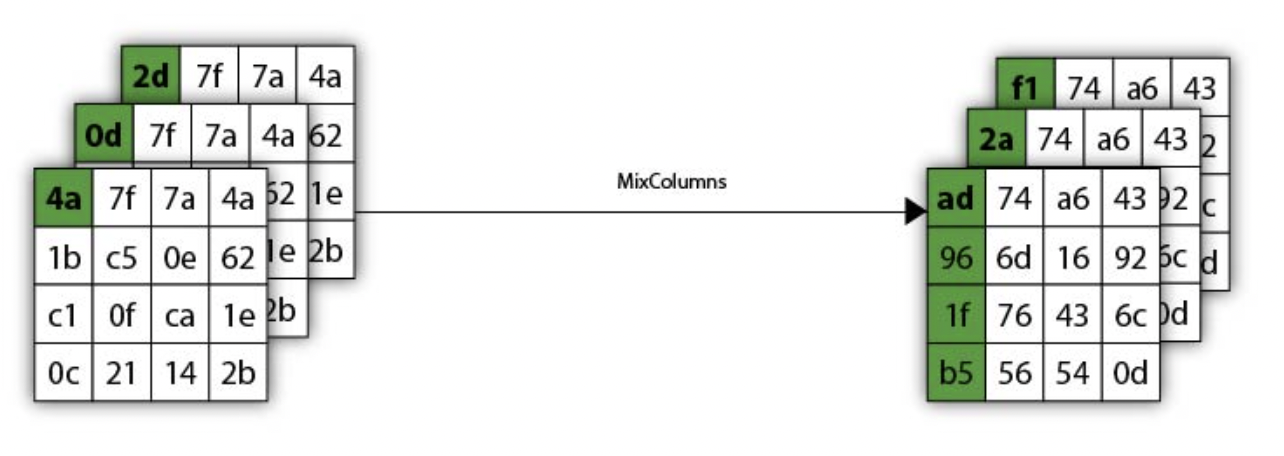
\includegraphics[scale= 0.3]{deltaset3}
\end{center}
Quando parliamo di "attivazione di cella" intendiamo che l'effetto della cella inizialmente attiva va ad influire sul valore di tutte le altre, la proprietà di $\Delta$ set è quindi presente su 4 celle attive. L'indice di una cella è considerata attiva se la cella può assumere tutti i differenti valori di un byte all'interno di un set di 256 differenti plaintexts. Contrariamente una cella è considerata inattiva se prende lo stesso valore all'interno del set di plaintexts.
\subsubsection*{Confusion and diffusion}
Se ci concentriamo sulla situazione alla fine del secondo round possiamo vedere che la proprietà di $\Delta$ set è ancora presente questa volta tuttavia è presente su tutte le celle.
\begin{center}
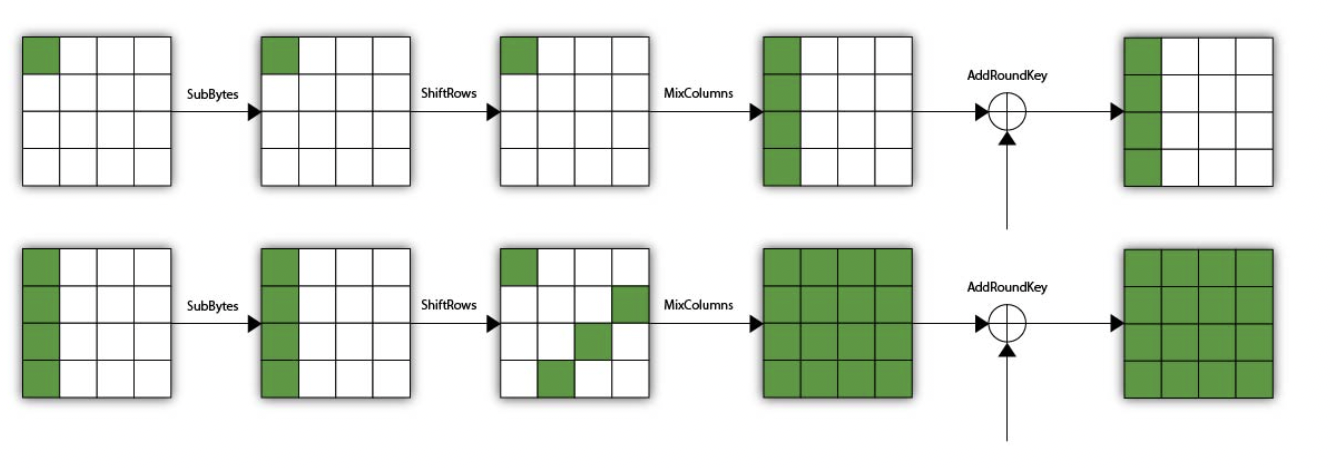
\includegraphics[scale= 0.4]{deltaset4}
\end{center}
Possiamo inoltre intuire che dal terzo round di AES la proprietà di $\Delta$ set è persa.\\
Possiamo concludere che una variazione nel plaintext o della chiave va ad influire in maniera esponenziale sul ciphertext, questa proprietà è chiamata confusion e diffusion, ovvero che tutto dipende da tutto.
\subsubsection*{Attacco ad AES}
\begin{center}
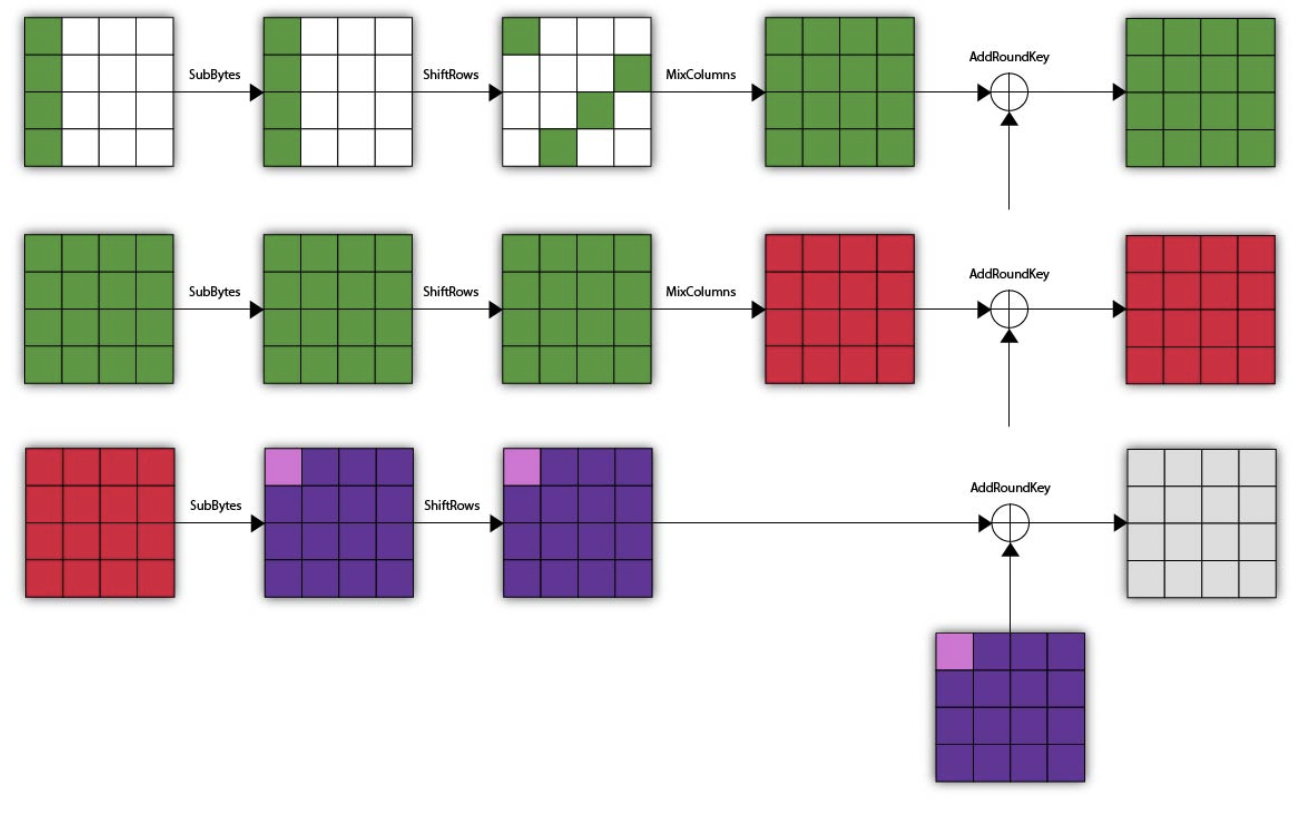
\includegraphics[scale= 0.4]{deltaset6}
\end{center}
Se eseguiamo un ulteriore round di AES possiamo notare che l'output non possiede la proprietà di $\Delta$ set, sorge tuttavia uno scenario di attacco, in particolare possiamo prendere una cella del round di output, ed effettuare un attacco di tipo bruteforce della chiave. Se il valore mi restituisce di nuovo un $\Delta$ set possiamo essere certi di aver ritrovato la porzione di chiave corretta; questa operazione è svolta su tutte le celle, una alla volta, fino a ricavare la chiave intera.

\long\def\comment#1{
\emph{review}
\begin{figure}[H]
\begin{subfigure}[h]{0.5\linewidth}
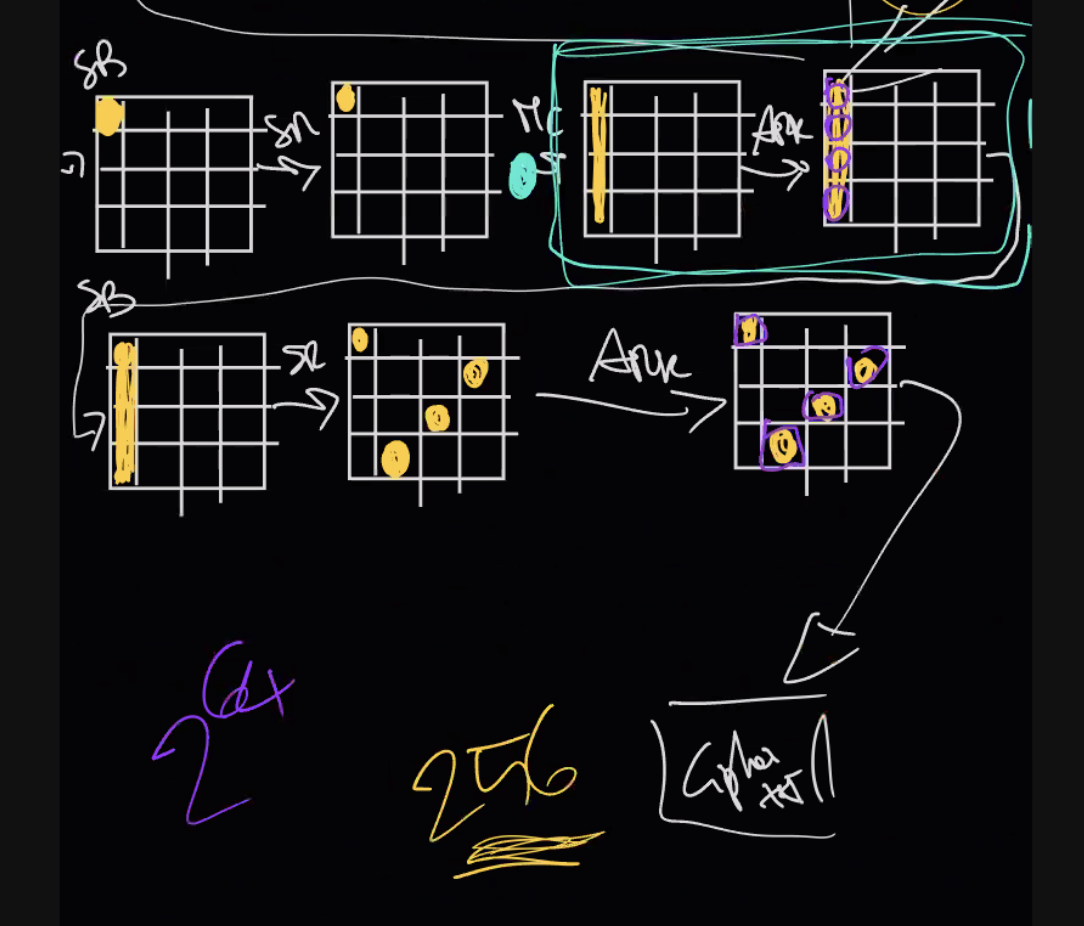
\includegraphics[width=\linewidth]{rev}
\end{subfigure}
\hfill
\begin{subfigure}[h]{0.5\linewidth}
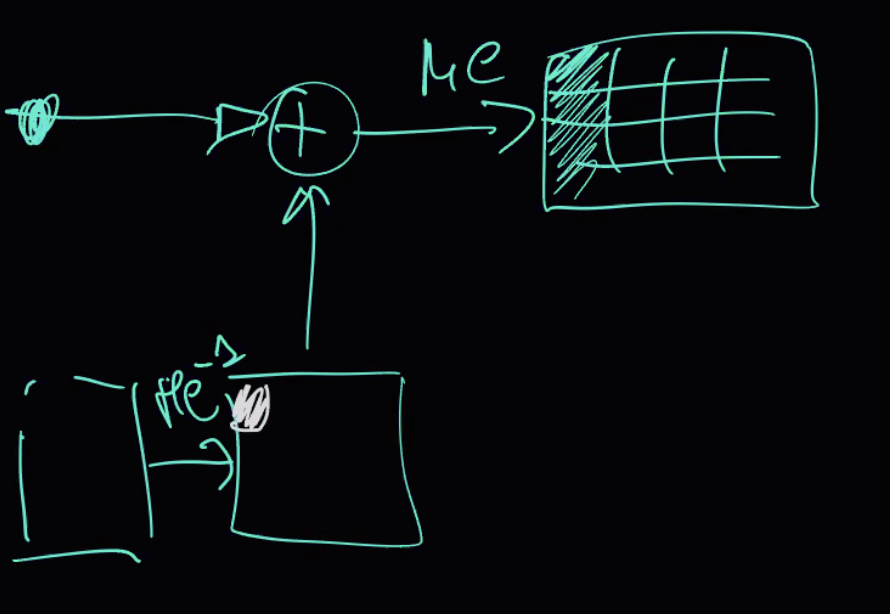
\includegraphics[width=\linewidth]{rev2}
\caption*{il pallino è la chiave, mi serve solo il primo byte della chiave}
\end{subfigure}%
\end{figure}
Lo sforzo computazionale è sceso da $2^{64}$ a $2^8* 5 = 2^{40}$, uno nel penultimo round, 4 nei round.
Per 5 round lo sforzo computazionale è $2^{32} * 2^{40} = 2^{72}$.
}



\section*{Crittografia asimmetrica}
Come abbiamo visto in precedenza, la crittografia asimmetrica differisce dalla crittografia simmetrica in quanto entrano in gioco ulteriori chiavi, ovvero le chiavi private. Le chiavi che entrano in gioco nei processi di cifratura e decifratura sono quindi differenti. \\Le chiavi nella crittografia asimmetrica sono di piccola grandezza, in quanto il mantenimento comporta uno sforzo computazionale non indifferente
\begin{center}
Encryption: $E_{pub}(M) = C$ \\
Decryption: $D_{priv}(C) = M$ 
\end{center}
Il processo di scambio di chiavi pubbliche avviene attraverso un processo di \emph{handshake}.
\section*{RSA}
E' un algoritmo di cifratura asimmetrica introdotto negli anni 70, il nome proviene dal nome degli inventori (Rivest-Shamir-Adleman).\\
L'algoritmo di RSA è suddivisibile in 4 macro-fasi: la generazione della chiave, la distribuzione della chiave, l'encryption e la decryption. La chiave pubblica è conosciuta da chiunque, ed è utilizzata da Bob per cifrare di messaggi mentre la chiave privata è conosciuta solo da Alice è utilizzata per decifrarli.
E' un cifrario a chiavi pubbliche ed i principali parametri sono:
\begin{itemize}
\item le chiavi pubbliche: $public(n,e)$:\\
- (solitamente) $e = 2^{16}+1 = 65.537$\\
- $n = p * q$
\item le chiavi private: $private(p,q,d)$:\\
- $p$ e $q$ sono due numeri (segreti) primi arbitraria grandi, in genere $>$ 1024 bit.\\
Questi valori devono essere grandi, per fornire un alto grado di entropia\\
- $d * e = 1$ $mod(\phi(n))$ (d segreto)
\end{itemize}
In particolare il valore $\phi(n)$ è chiamata funzione "phi" di Eulero, e rappresenta l'insieme dei numeri $k$ nel range di $1 \leq k \leq n$ per cui il massimo comune divisore è 1, ovvero
\begin{center}
$k$ in $1 \leq k \leq n$ t.c. \\
gcd(n, k) = 1\end{center}
Possiamo infine riscrivere $\phi$ nel seguente modo:
\begin{center}
$\phi = (p-1)(q-1)$
\end{center}

\begin{itemize}
\item $e$ è un numero casuale tale che $MCD(e, \phi(n)) = 1$
\end{itemize}

Le componenti pubbliche sono $n$ ed $e$, mentre le componenti private sono $p, d, e$
\subsection*{Funzionamento di RSA}
\begin{enumerate}
\item Generiamo due numeri primi $p, q$ (sulla quale effettuiamo un controllo di adeguatezza applicando gli algoritmi di Euclide esteso, Fermat, Miller Rabin e Pollard) di grandezza simile, arbitrariamente grande per calcolare un numero $n$ tale che $n = p \times q$ sia sufficientemente grande, in genere di grandezza $> 1024 bit$. 
\item Calcoliamo $n = p \times q$ e $\phi = (p - 1)(q - 1)$
\item Selezioniamo un valore $e$, tale che $1 < e < \phi$ e tale che $gcd(e, \phi) = 1$
\item Calcoliamo l'esponente segreto $d$, tale che $1 < d < \phi$ e tale che $ed \equiv 1$ $mod$ $\phi$ 
\end{enumerate}
\begin{center}
la chiave pubblica è $(n, e)$\\
la chiave privata è $(d, p, q)$
\end{center}
Alice per effettuare la fase di encryption: \begin{center}
$M^{e} = C$ $mod$ $n$ ove $M$  $<$ $n$
\end{center}
Bob per effettuare la fase di decryption: \begin{center}
$C^d = M$ $mod$ $n$
\end{center}

\subsection*{Il valore e}
Il valore $e$ può essere un valore casuale, che tuttavia deve essere scelto tale che valga la seguente condizione $MCD(e, \phi(n))=1$ (con l'applicazione dell'algoritmo di Euclide)
\subsubsection*{Ma perché viene scelto $2^{16}+1$ solitamente?}
Consideriamo dove viene applicato: 
\begin{center}
$N^e$ mod $n$
\end{center}
Il valore $2^{16} = 65537$ in codifica binaria è: $10000000000000001$\\
Possiamo vedere che nella compaiono molti 0, e pochi 1, questo ci permette di effettuare operazioni di esponenziazione modulare più veloce, avendo solo 2 bit con valore 1.
Il valore è in particolare $e$ perché deve essere coprimo con $d$, verificabile calcolando l'inverso moltiplicativo \\
Il valore 65537 è scelto perché è un valore sufficientemente grande, che supera di un numero arbitrario di volte la $n$ nel modulo, aumentando lo sforzo computazionale richiesto al momento del calcolo della radice. In particolare quando andiamo a fare il bruteforcing, più grande è il valore $e$, più alto il valore che dobbiamo bruteforcare
\subsection*{Il valore d}
Il valore $d$ è calcolato utilizzando l'algoritmo esteso di Euclide per calcolare \begin{center}
$d = e^{-1}$ $mod$ $\phi$ oppure\\
$d = \frac{1}{e}$ $mod$ $\phi$
\end{center}
Ovvero l'inverso modulare. Notare come questo non è la divisione classica, ma l'inverso modulare $d$ è definito come valore intero tale che $ed = 1$ $mod$ $\phi$, che esiste sse $e, \phi$ sono coprimi.

\subsection*{Per applicare l'algoritmo RSA abbiamo bisogno di alcuni strumenti:}
\begin{itemize}
\item l'algoritmo di Euclide per l'MCD di due valori interi, per verificare se questi sono coprimi. (Utilizzato durante la determinazione di $p, q$)
\item l'algoritmo di Euclide esteso per la determinazione dell'inverso moltiplicativo
\item il teorema piccolo di Fermat per la verifica di primalità
\item la generalizzazione del teorema piccolo di Fermat ovvero il teorema di Eulero per l'euler totient ($\phi(n)$.
\item Il teorema cinese dei resti per lo scaricamento dello sforzo computazionale su server

\end{itemize}

\subsection*{Coprimi: "l'algoritmo di Euclide" e "piccolo teorema di Fermat"}
Per verificare che due valori a, b siano coprimi, ovvero che $MCD(a, b)=1$ possiamo:
\begin{itemize}
\item Per valori non troppo grandi: per fattorizzare due valori a, b arbitrariamente grandi dobbiamo verificare tutti i numeri primi fino a radice di a. 
\item Per valori grandi utilizzare \emph{l'algoritmo di Euclide}
\end{itemize}
\subsection*{L'algoritmo di Euclide per il calcolo dell'MCD}
L'algoritmo di Euclide è un algoritmo efficiente utilizzato per calcolare l'MCD di due valori interi, senza conoscere nulla sui divisori dei due valori. Se l'output dell'algoritmo di Euclide per due valori $a,b$ è 1 allora possiamo concludere che due valori sono coprimi.
\begin{center}
$a = bq_1 + r_1$\\
$b = r_1 q_2 + r_2$\\
$r_1 = r_2q_3 + r_3$\\
...\\
$r_{k-2} = r_{k-1}q_k+r_k$\\
$r_{k_-1} = r_kq_{k+1} + 0$\\
\end{center}
Se ci troviamo in questa situazione l'algoritmo di Euclide ha trovato resto uguale a 0.\\
L'MCD è quindi $MCD(a,b) = r_k$\\
Proviamo a fare il calcolo con $a = 1180, b= 482$
\begin{center}
$1180 = 482*  2 +216$\\
$482 = 216*2+50$\\
$216 =50*4+16$\\
$50=16*3+2$\\
$16=2*8+0$
\end{center}
Possiamo concludere che $l'MCD(1180, 482) = 2$


\subsection*{L'algoritmo di Euclide esteso per l'inverso moltiplicativo}
\begin{center}
consideriamo $MCD(a,b) = ax+by$\\
\end{center}
\emph{Come calcoliamo x e y?}\\
Partiamo da x:\begin{center}
$x_0 = 1$\\
$x_1 = 0$\\
$x_2 = -q_{j-1} * x_1+x_0$\\
...\\
$x_j = -q_{j-1} * x_{j-1} + x_{j-2}$
\end{center}
Per calcolare y invece: \begin{center}
$y_0 = 0$\\
$y_1 = 1$\\
...\\
$y_j = -q_{j-1}*y_{j-1}+y_{j-2}$
\end{center}
Considerando $MCD(1180,482) = 2 = 1180y+482x$
\begin{center}
$x_0 = 1$\\
$x_1 = 0$\\
$x_2 = -2(1)+0 = -2$\\
$x_3 = -2(-2)+1= 5$\\
$x_4 = -4(5)-2 = -22$\\
$x_5 = -3(-22)+5 = 71$\\
Ricaviamo che $x = 71$\\
\end{center}
\begin{center}
$y_0 = 0$\\
$y_1 = 1$\\
$y_2 = -2(0)+1 = 1$\\
$y_3 = -2(1)+0= -2$\\
$y_4 = -4(-2)+1 = 9$\\
$y_5 = -3(9)-2 = -29$\\
Ricaviamo che $y=-29$
\end{center}
Allora abbiamo che $MCD(1180,482) = -29(1180) + 71(482) = 2$\\\\
L'inverso moltiplicativo deve essere $= 1$, ovvero $ax+by =MCD(a,b)=1$
Poniamo noi l'inverso moltiplicativo =1 perché il processo di decifratura è unica, se avessimo 2 ci sarebbero più decifrature possibili
\begin{center}
$by \equiv 1$ mod $a$\\
$by \equiv 1 + tot * a$ ove $tot = x$\\
$y*b = 1$ mod $a$
\end{center}


\subsection*{Teorema piccolo di Fermat ed il teorema di Eulero}
Il teorema piccolo di Fermat dice che se $p$ è un valore primo, per ogni intero $a$, il valore $a^p-a$ è un intero multiplo di $p$.
\begin{center}
$a^p \equiv a$ $(mod$ $p )$  oppure  $a^{p-1}\equiv 1$ $(mod$ $p )$
\end{center}
Attraverso il \emph{teorema di Eulero} possiamo generalizzare il teorema di Fermat, in particolare: per ogni modulo $n$ ed ogni intero $a$ coprimo rispetto a $n$ abbiamo:
\begin{center}
$a^{\phi(n)} \equiv 1$ $(mod$ $n)$
\end{center}
Ove $\phi(n)$ rappresenta la funzione di Eulero, che conta il numero di interi fra 1 e $n$ coprimi rispetto ad n. Se $n = p$ è un numero primo allora 
\begin{center}
$\phi(p) = p-1$
\end{center}
Vediamo un esempio di applicazione del piccolo teorema di Fermat.\\
Supponiamo di voler calcolare $2^{43210}$ $mod$ $101$.
\begin{center}
Trasformiamo l'esponente: $43210$ in  $432*100 + 10$\\
$(2^{100})^{432}  * 2^{10}$ mod $101$\\ 
Teorema di Fermat: \\$a^{p-1}\equiv$ mod $p$\\
Allora $1^{432} * 2^{10} $ mod 101\\
Infine: $1024$ mod $101 = 14$
\end{center}

\subsection*{Considerazioni su modulo ed esponente}
Consideriamo $a, n, x, y$ numeri interi, $n \geq 1$ t.c. $MCD(a,n) = 1$ \\
Dimostriamo che se lavoriamo con le basi stiamo lavorando con $mod$ $n$, mentre se stiamo lavorando con gli esponenti lavoriamo con $\phi(n)$.
\begin{center}
se $x = y$ $mod$ $\phi(n)$\\allora $a^x = a^y$ $mod$ $n$
\end{center}
In particolare possiamo dire che $x = y$ $mod$ $\phi(n)$ se esiste un intero $k$ per cui vale la seguente proprietà:
\begin{center}
$x = y + k\phi(n)$
\end{center}
Di conseguenza:
\begin{center}
$a^x = a^{y + k \phi(n)} = a^y * (a^{\phi(n)})^k$
\end{center}
Applicando il teorema di Eulero Fermat possiamo fare la seguente operazione: 
\begin{center}
$a^{\phi(n)} = 1$ $mod$ $n$\\
$a^y * (a^{\phi(n)})^k$ diventa $a^x = a^y * 1^k$ $mod$ $n$
\end{center}
Ma siccome $1^k$ è irrilevante, possiamo eliminarlo e rimaniamo con $a^x = a^y$. Concludiamo quindi che $\phi(n) = \phi(p) = p-1$




\section*{Attacking RSA}
Siccome il cifrario RSA è stato introdotto nel 1970, durante gli anni sono stati eseguiti numerosi attacchi, che vertono sulle problematiche algoritmiche, matematiche ed ingegneristiche. 
\subsection*{$\phi$(n) accessibile}
Consideriamo un caso in cui l'attaccante sia in grado di accedere al valore $\phi(n)$, magari attraverso ad un dump della memoria dopo che un programmatore l'ha utilizzato, senza cancellare il valore. Siccome i valori della chiave pubblica sono $(n, e)$, abbiamo i seguenti valori disponibili: $(n, e, \phi)$. Se effettuiamo:
\begin{center}
$n-\phi(n)+1 =$\\
$=pq-[(p-1)(q-1)]+1=$\\
$=pq-[pq-p-q+1]+1=$\\
$=p+q$
\end{center}
Deduciamo che se troviamo $\phi$ possiamo ricavare $p+q$. \\Consideriamo ora che $n=p*q$ e $\phi(n) = (p-1)(q-1)$
\begin{center}
$ax^2+bx+c$ \\ove $c = p*q = n$, $a =1$, $b = p+q$\\
$x_1x_2 = c/a$\\
$x_1+x_2 = -b/a$
\end{center}
Possiamo quindi ricavare che\begin{center}
$x^2-x(n-\phi(n)+1)+n=0$\\
Se risolviamo con il $\Delta$ possiamo ricavare i valori $x_1 = p $ e $x_2 = q$
\end{center}

\long\def\comment#1{
\subsection*{Caso valido su d}
Riguardareeeeee
\begin{center}
Se MCD(a,n) = 1
Allora esiste un vlore s,t tle che s >= 0; t > 0
Allora in questo caso esiste 
\end{center}
}


\subsection*{Casi particolari su d}
Per l'algoritmo di Euclide esteso abbiamo imposto come condizione che \begin{center}
$MCD(a,n) = d = 1$
\end{center}
Ma cosa succede se non fosse così?
\begin{center}
$MCD(a,n) = d \neq 1$\\
$ax \equiv b$ $mod$ $n$
\end{center}
Possiamo dire che:\begin{itemize}
\item se d non divide b, allora non esiste soluzione per $ax \equiv b$ $mod$ $n$
\item se d divide b, allora esiste soluzione per $ax \equiv b$ $mod$ $n$, ma non è unica, la congruenza iniziale avrà $d$ soluzioni. Per decifrare provare più soluzioni, scartando quelle che non mi interessano
\begin{center}
$ax \equiv b$ $mod$ $n$\\
$ax/d \equiv b/d$ $mod$ $n/d$
\end{center}
Chiamiamo la prima soluzione $x_0$, per calcolare le successive soluzioni possiamo
\begin{center}
$x_0 + n/d$, $x_0 + 2n/d$ ,..., $(d-1)(n/d)$
\end{center}
Le soluzioni sono quindi $(d-1)$

\end{itemize}

\subsection*{Attacchi da conoscere a carattere informativo:}

\subsection*{Caso m/4 cifre esposte di p, q, d}
Supponiamo di avere\begin{center}
$n = p * q $ di $n$ cifre
\end{center}
Se siamo in grado di recuperare le prime $m/4$ cifre di $p$ o di $q$ esiste un attacco in tempo polinomiale in grado di fattorizzare $n$. Questo attacco è stato successivamente esteso, in particolare se sono in grado di recuperare le prime $m/4$ cifre di $d$  sono ancora una volta in grado di rompere RSA


\subsection*{Low exponent attacks}
Consideriamo $(e,n)$, \begin{center}
$d* e \equiv 1$ $mod$ $\phi(n)$, con d$\in [1, ..., \phi(n)]$\\
Se $d < 1/3\sqrt[4](n)$
\end{center} 
Esiste un algoritmo in grado di attaccare la chiave in pochi millisecondi

\subsection*{Common modulus attack}
Consideriamo:
\begin{center}
$Alice = (e_A, n)$ | $Bob = (e_B, n)$
\end{center}
Cosa succede se sia Alice che Bob utilizzano uno stesso $p,q$, e di conseguenza $n$?
\begin{center}
$M^{e_A} = C_1$ $mod$ $n$\\
$M^{e_B} = C_2$ $mod$ $n$
\end{center}
Consideriamo un terzo soggetto Carl, che deve inoltrare un messaggio ad Alice e Bob, cifra i messaggi:
\begin{center}
Crittotesto per Alice: $M^{e_A} = C_1$ $mod$ $n$\\
Crittotesto per Bob: $M^{e_B} = C_2$ $mod$ $n$
\end{center}
Se Eve è in grado di recuperare i crittotesti $C_1$ e $C_2$, e nota che gli $n$ di Bob e Alice sono congruenti
\begin{center}
$(C_1^{-1})^{-r} * (C_2)^s=$\\
$= ((M^{e_{a}})^{-1})^{-r} * (M^{e_b})^s =$\\
$= M^{e_{a}r} * M^{e_{b}s}$
\end{center}
Noi tuttavia sappiamo che è valida la seguente congruenza: $1 \equiv e_a r + e_b s$ $mod$ $\phi(n)$
E posisamo sostituirla all'esponente, rimaniamo quindi con:
\begin{center}
$= M^{e_{a}r} * M^{e_{b}s} =$\\
$m^1$ $mod$ $n$\\
$m$
\end{center}
Come possiamo vedere Eve è stata in grado di recuperare il messaggio $m$ sfruttando una vulnerabilità $n$ comune

\subsection*{Short plaintext attack}
Attacco probabilistico attuabile nel caso in cui un plaintext sia troppo piccolo, in particolare un plaintext cryptato con DES avrà ordine di grandezza di $m = 10^{17} \equiv 2^{56}$. Il valore $m$ è ri-scrivibile come \begin{center}
$m = a*b$
\end{center}
$a,b$ avranno, con una probabilità non trascurabile, un ordine di grandezza di $10^9$ (valore preso accettabile per un computer diffuso)
Li suddivido ora in due array di $10^9$ elementi, in particolare ricavati rispettivamente con
\begin{center}
$array_1$ = $c*x^{-e}$ $mod$ $n$\\
$array_2$ = $y^e$ $mod$ $n$\\
Con $x, y$ che sono gli indici negli array
\end{center}
\begin{center}
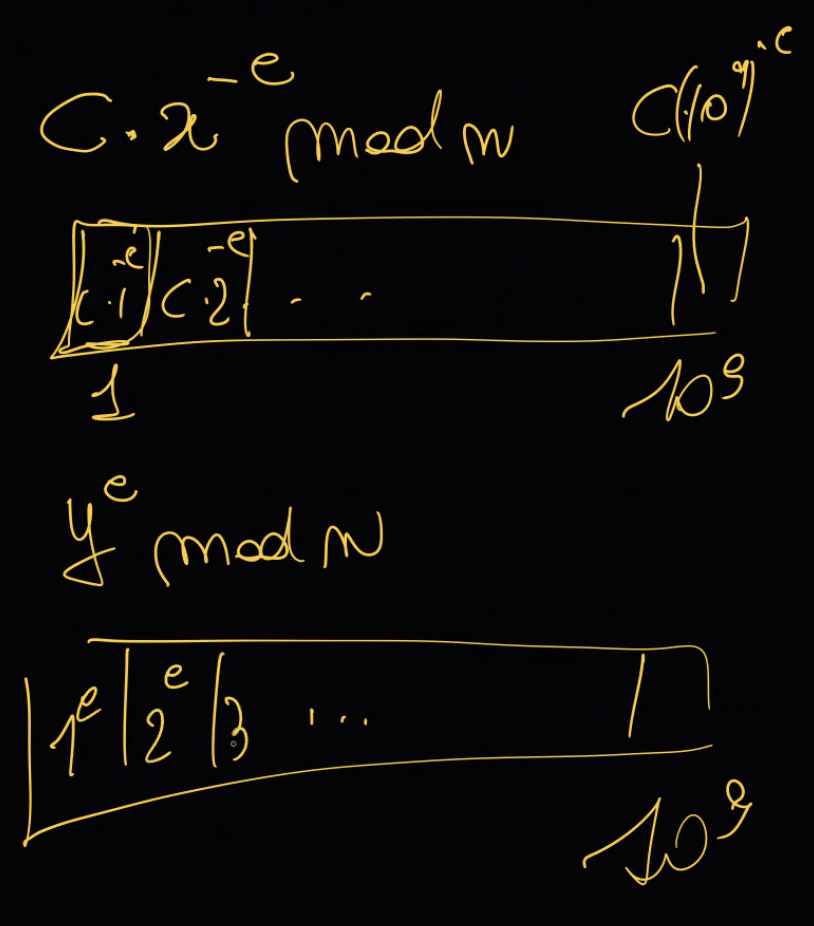
\includegraphics[scale= 0.4]{m1}
\end{center}
In una posizione arbitraria in ogni array sarà possibile trovare 2 celle con lo stesso valore, uguagliando il contenuto dei due array è possibile ricavare il messaggio.
\begin{center}
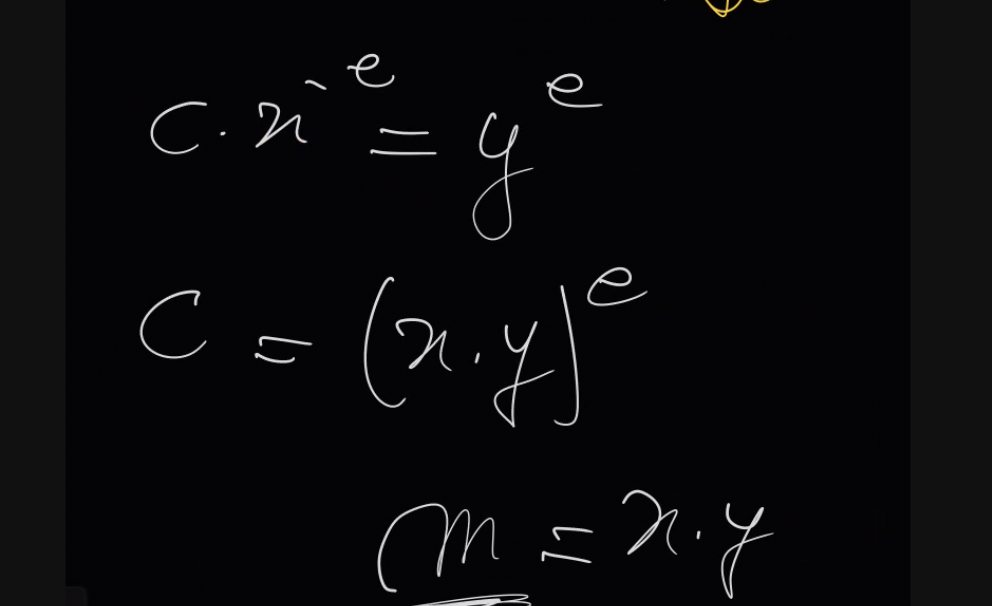
\includegraphics[scale= 0.4]{m2}
\end{center}
In particolare ho trovato i fattori $x * y$, ricavando cosi il valore $m$

\subsection*{Padding per short plaintexts | OAEP}
Per raggirare il problema di plaintext troppo corto viene aggiunto un padding, ovvero una stringa definita, inserita in coda al plaintext. In particolare per RSA viene utilizzato l'\emph{OAEP} (optimal asymmetric encryption padding), il cui valore è generato da una funzione Feistel (la parte della generazione del padding è ignorata). Per criptare plaintext corti, quindi, viene generato un padding di lunghezza $x$.\\
Dato un messaggio troppo corto $M$ di lunghezza $i$, il messaggio unito col padding $P$ con lunghezza $k$ diventa:	\begin{center}
$M_i \rightarrow$ $M_iP_k$

\end{center}
$M_iP_k$ è poi utilizzato per produrre il ciphertext


\subsection*{Teorema cinese dei resti}
Permette di fare il calcolo dell'inverso attraverso la risoluzione di sistemi, che permette di scaricare il carico computazionale al server\\
Consideriamo un set di numeri interi o naturali:
\begin{center}
$for$ $i$ 	$P_i/Z_i = r_1r_2...r_{i-1}r_{i}$\\
$for$ $i$ 	$Q_i/Y_i = Z^{-1}_i$ $mod$ $r_i$\\
$x = a_1y_1z_1+ ... + a_ny_nz_n$\\
\end{center}
Questo viene fatto perché il calcolo dell'inverso moltiplicativo nel metodo tradizionale è un'operazione dispendiosa. La risoluzione del sistema risulta meno dispendiosa, e ci permette anche a scaricare il server ad un'altra location.
\subsection*{Lemma del teorema cinese dei resti}
Consideriamo due interi $m, n$ coprimi fra loro, ovvero:
\begin{center}
$m,n$ t.c. $MCD(m,n) = 1$
\end{center}
Se $c$ un altro intero è multiplo di $m$ e $n$ \begin{center}
ovvero $c = m*k$, $c = n*l$\end{center}
 allora 
 \begin{center}
 $c$ è multiplo di $(m*n)*x = c$
 \end{center}
 
 
 \long\def\comment#1{
\subsection*{Lemma del teorema cinese dei resti}
Consideriamo:\begin{center}
$(m^e)^d = m$ $mod$ $n$
\end{center}
Consideriamo 2 dei 4 casi possibili su $m$
\begin{center}
$MCD(p,m) \neq 1 = d$
\end{center}
Allora $p$ ed $m$ hanno qualcosa in comune, in particolare $d=  p$ , e $p | m$, di conseguenza
\begin{center}
$M \equiv 0$ $mod$ $p$\\
Consideriamo $e*d = 1$ $mod$ $\phi(n)$\\
$M^{ed} \equiv M^{k(p-1)(q-1)+1}$ $mod$ $p$\\
\end{center}
\emph{TO REVIEW}
}

\subsection*{Timings attacks}
Un attacco notato per la prima volta da uno studente della Stanford 20 anni dopo l'implementazione di RSA. Questo attacco espone informazioni private misurando l'ammontare di tempo richiesto o analizzando l'oscillazione durante le operazioni svolte sulla chiave privata.\\
Possiamo raggirare questa problematica offuscando l'implementazione, rendendo il tempo d'esecuzione costante (per esempio introducendo una serie di nop), in alternativa attraverso la tecnica di sliding windows, si effettuano i calcoli su un subset di bits. 

\section*{Chiavi RSA}
Consideriamo i valori $p,q$, due numeri primi, abbiamo detto che questi valori devono essere arbitrariamente grandi per garantire un buon grado di sicurezza\\
\emph{Ma come verifichiamo che un numero sia adatto?}\\
Siccome non possiamo utilizzare un algoritmo deterministico per determinare la conformità di $n$, in quanto il calcolo dei numeri primi non è deterministico, utilizziamo un approccio probabilistico. Andiamo a verificare il valore $n$ con una serie di test per escludere valore inadatti.\\
In modo per determinare un valore $n$ adatto è il seguente:
\begin{itemize}
\item determiniamo un lower bound di $10^{100}$, determiniamo un valore $P_0 \cong10^{40}$
\item verifichiamo con $P_0$ con Miller Rabin
\item determiniamo un valore $k$ tale che $P_o * k$ $\cong$ $10^{100}$, $k$ sarà dell'ordine di $10^{60}$
\item $p_0 * k+1 = p$, applichiamo Miller Rabin $n$ volte, se passa, $p$ è primo
\end{itemize}
Questo ci permette di evitare l'attacco di Pollard in quanto il valore è $p-1$ è sicuramente un valore non basso.
\subsection*{Test di primalità di Fermat}
Consideriamo
\begin{center}
$n, x, y$ tale che $x^2 \equiv y^2$ $mod$ $n$\\
se $n \neq \pm y \rightarrow$ $n$ è composto
\end{center}
In particolare
\begin{center}
$MCD(x-y; n)$ fornisce un fattore di $n$
\end{center}
Consideriamo ora \begin{center}
$n$ un intero arbitrariamente grande\\
$\pm a < n-1$\\
se $a^{n-1} = d$ $mod$ $n$\\
Ovvero che $a^{n-1} \neq 1$ $mod$ $n$
\end{center}
allora possiamo concludere che $n$ è  un numero composto, per il piccolo teorema di Fermat.
se invece: 
\begin{center}
se $a^{n-1} = 1$ $mod$ $n$
\end{center}
Non possiamo concludere nulla su $a$. Il teorema piccolo di Fermat è quindi utilizzato per verificare che un numero è composto.\\

Siccome non siamo stati in grado di determinare nulla su $a$, utilizziamo un altro test, in particolare 
il test di Miller-Rabin
\subsection*{Test di primalità di Miller Rabin}
Consideriamo un valore primo dispari $n$ da verificare
\begin{center}
$n-1 = 2^k * m$
\end{center}
Consideriamo: 
\begin{center}
$a < n-1$\\
\end{center}
Andiamo ad applicare l'algoritmo di Miller Rabin
\begin{center}
$b_0 = a^m$ $mod$ $n$
\end{center}
Se $b_0$ è uguale a \begin{itemize}
\item +/- 1 allora $n$ è probabilmente primo
\item altro, allora proseguiamo con $b_1$
\end{itemize}
\begin{center}
$b_1 = b^2_0$ $mod$ $n$
\end{center}
Se $b_1$ è uguale a \begin{itemize}
\item +1 allora $n$ è composto
\item -1 allora $n$ è probabilmente primo
\item altro, allora proseguiamo con $b_2$
\end{itemize}
In particolare $b_2$ viene calcolato nella stessa maniera in cui è calcolato $b_1$, elevando alla seconda il valore $b_{m-1}$ e modulando.\begin{center}
$b_k = (b_{m-1})^2$ $mod$ $n$
\end{center}
L'algoritmo termina quando calcoliamo il valore $b_{k-1}$, in particolare se $b_{k-1}$ è uguale a \begin{itemize}
\item +1 allora $n$ è composto
\item -1 allora $n$ è probabilmente primo
\item altro, allora scegli un altro valore $n$ da verificare
\end{itemize}
L'algoritmo di Miller Rabin ha una probabilità di errore del 25\%, un risultato su 4 è errato. 

Tuttavia 25\% non è soddisfacente, per mitigare la probabilità l'algoritmo di Miller Rabin è applicato più volte su $j$ valori diversi, in particolare se la probabilità è 25\% per una verifica, per 10 verifiche la probabilità di errore diventa
\begin{center}
$(1/4)^{10}$
\end{center}
I valori che passano il test di Fermat sono chiamati \emph{pseudoprimi}, mentre quelli che passano sia Fermat che Miller Rabin sono chiamati \emph{pseudoprimi forti}
Consideriamo \begin{center}
$n = 13 \rightarrow n-1 = 12 = 2^2*3$
prendiamo a = 11\\
$b_0 = 11^3$ $mod$ $13$
$b_0  = 5$
$b_1 = 25 mod 13 -> 12$
$b_2 = 144 mod 13$
\end{center}
Le banche utilizzano Fermat, Miler Rabin, Solovay–Strassen per effettuare test di primalità.


\subsection*{Fattorizzazione di n}
Dato un valore $n$ composto, come possiamo fattorizzarlo nei valori $p, q$?
Introduciamo la tecnica di fattorizzazione di Fermat. Consideriamo $n,i,j$ tale che
\begin{center}
$n+i^2 = j^2$
\end{center}
Allora possiamo fattorizzare $n$, infatti:
\begin{center}
$n = j^2 - i^2=$\\
= (j+i)(j-i)
\end{center}
Ad esempio consideriamo $n = 295927$
\begin{center}
$n+1^2 = j^2$
\end{center}
se è possibile abbiamo finito, senò proseguiamo:
\begin{center}
$n+2^2 = j^2$\\
$n+3^2 = 295936 = 544^2$\\
$n = (544+3)(544-3)=$\\
$n = 547 * 541$
\end{center}
Abbiamo trovato che $p = 547, q = 541$. La difficoltà sta nel trovare i valori $i, j$, in quanto la ricerca di tali valori è lenta.
\subsection*{Fattorizzazione di n | algoritmo di Pollard}
Consideriamo\begin{center}
$n = p * q$
\end{center}
Se è possibile scriver $p-1$ come un prodotto di numeri primi piccoli, allora il valore $p$ è facilmente attaccabile con l'algoritmo di Pollard. Ad esempio:
\begin{center}
$p-1 = 2^{101} * 3^7 * 5^{10} * 7^ {701}$
\end{center}
Come possiamo vedere i tali valori sono "piccoli", il valore $p$ non è adatto.

\subsection*{Quadrato di Sieve}
Il quadrato di Sieve è un algoritmo per la fattorizzazione (sieve = setaccio).
Consideriamo \begin{center}
$n = p * q$
\end{center}
Selezioniamo $k$ valori su cui applicare $mod$ $n$.
\begin{center}
$123456 ^2$ $\equiv x$ $mod$ $n$ 
\end{center}
Supponiamo che $x = 2^3*3^4*11*23^2$, continuiamo provando con $n$ valori $x_n$

\begin{center}
$n = 3837523$
\end{center}
Selezioniamo $k$ valori su cui applicare $mod$ $n$, più valori scegliamo , più precisa sarà la nostra stima. Ad esempio scegliamo 9398, 19095, 1964, 17078
\begin{center}
$9398^2 = 5^5 * 19$ $mod$ $n$\\
$19095^2 = 2^2 * 5 * 11 * 13 * 19$ $mod$ $n$\\
$1964^2 = 3^2 * 13^3$ $mod$ $n$\\
$17078^2 = 2^6 * 3^2 * 11$ $mod$ $n$\\
...
\end{center}
I valori a sinistra sono tutti valori al quadrato, moltiplicandoli tra di loro avremo sicuramente un valore quadrato, in particolare:
\begin{center}
$(9398 * 19095 * 1964 * 17078)^2$
\end{center}
Il valore all'interno delle parentesi lo chiamiamo $x$.
I valori a destra invece abbiamo $n$ valori con la stessa base, progressivamente moltiplichiamo tra loro e ricaviamo:
\begin{center}
$2^8*3^4*5^6*11^2*13^4*19^2$
\end{center}
Notiamo che tutti questi valori hanno una potenza quadrata, possiamo quindi riscriverla così:
\begin{center}
$(2^4*3^2*5^3*11*13^2*19)^2$
\end{center}
Il valore all'interno delle parentesi lo chiamiamo $y$.
\begin{center}
$x^2 \equiv y^2$ $mod$ $n$\\
Allora $n$ è composto e posso trovare uno dei due fattori di $n$ facendo: $x \neq \pm y\rightarrow$ $ (MCD(x-y; n) = d \neq 1$\\
Valore che è uguale a $p$ o $q$
\end{center}

\section*{Problema del logaritmo discreto}

\begin{center}
$\alpha^x \equiv \beta$ $mod$ $p$
\end{center}
Come faccio a trovare $x$? La cosa più intuitiva sarebbe utilizzare il logaritmo
\subsection*{Baby step giant step}
Il primo approccio è quello di utilizzare il \emph{baby step giant step}\\
Creiamo due vettori di grandezza $p$ (ovvero il modulo) in cui vengono inseriti gli elementi $\alpha_j$ nel primo vettore, $\beta\alpha^{-Nk}$ nel secondo vettore. Cerchiamo poi due valori comuni, per poi effettuare l'uguaglianza. 
\begin{center}
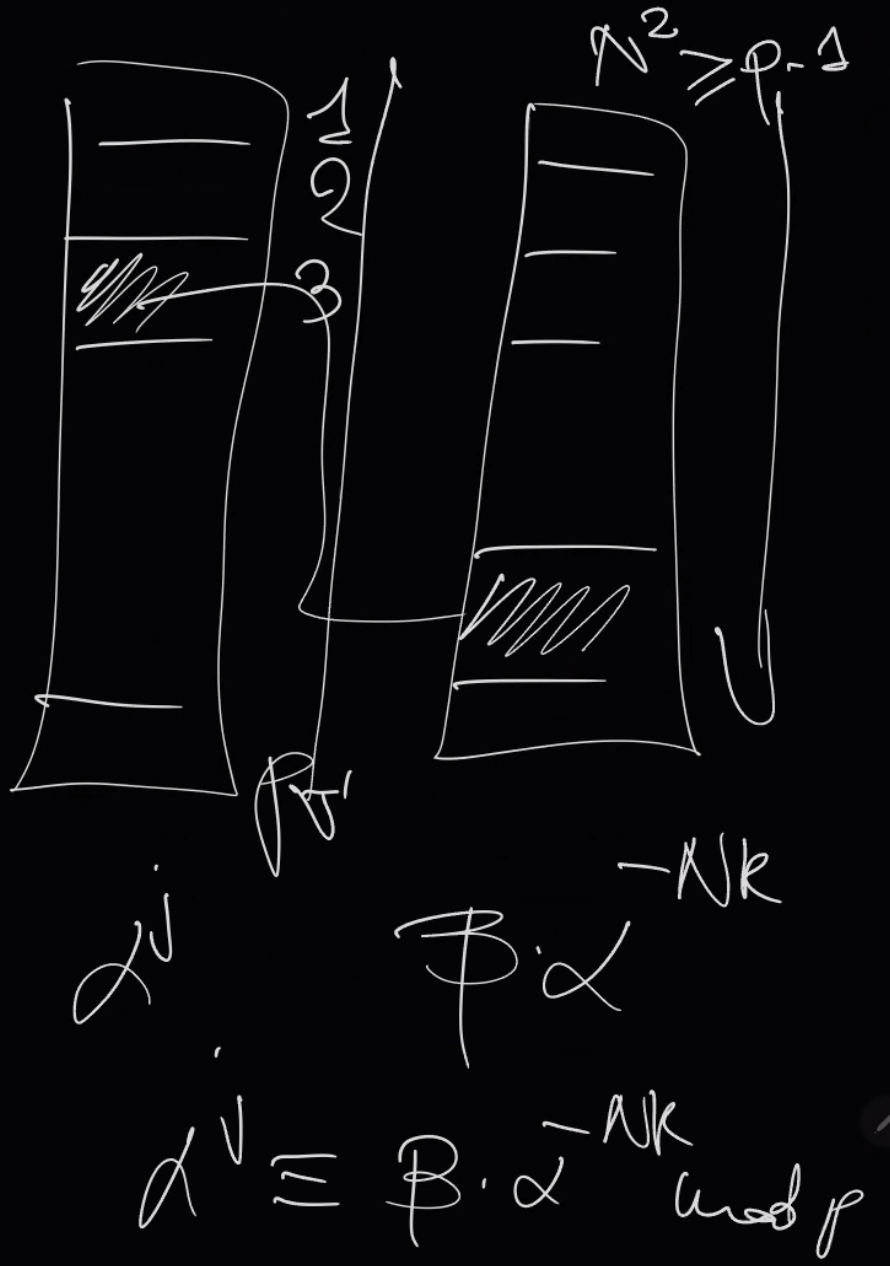
\includegraphics[scale= 0.4]{rev1}
\end{center}
In particolare l'uguaglianza
\begin{center}
$\alpha^j \equiv \beta * \alpha^{Nk}$ $mod$ $p$
\end{center}
E' uguale a 
\begin{center}
$\alpha^{j+NK} \equiv \beta$ $mod$ $p$
\end{center}
Ricordiamo che:
\begin{center}
$\alpha^x \equiv \alpha^y$ $mod$ $p$\\
$x \equiv y$ $mod$ $p-1$\\
$\alpha^{p-1}\equiv 1$ $mod$ $p$
\end{center}

\long\def\comment#1{
\subsection*{Analisi su parità o meno di x}
Possiamo inoltre dividere il sample size in 2, in particolare determinando se $x$ è pari o dispari.
}

\subsection*{Index calculus}
E' una variante del quadratic sieve basato su \begin{itemize}
\item un passo di precomputazione
\item calcolo dei logaritmi 
\item un passo di controllo proprietà, in particolare se è scomponibile
\end{itemize}
Consideriamo\\
\begin{center}
$\beta \equiv \alpha^x$ $mod$ $p$\\
$log_\alpha \beta = x$ $mod$ $(p-1)$
\end{center}
Consideriamo $a^k$ così definito:
\begin{center}
$a^k = \Pi p_i^{a_i}$ $mod$ $p$ ove $\Pi$ è la produttoria 
\end{center}
Allora il passo computazionale è il seguente:
\begin{center}
$k = log_\alpha (\Pi p_i ^{a_i})$
$= \sum a_i log_\alpha p_i$ $mod$ $p-1$
\end{center}
Questo ci permette di mettere in evidenza i logaritmi.
Il valore $\beta$ lo moltiplichiamo per un valore $a$ elevato ad un valore $r$ random, che ci permette di espanderlo nel seguente modo:
\begin{center}
$\beta * \alpha ^ r = \Pi p_i^{b_i}$ $mod$ $p$\\
$log_\alpha \beta + r log_\alpha \alpha = 
$=$ \sum b_i log_a p_i$ $mod$ $p-1$
\end{center}
Possiamo esporre quello che ci serve:
\begin{center}
$log_\alpha \beta = -r + \sum b_i log_a p_i$ $mod$ $p-1$
\end{center}
Abbiamo quindi trovato $x$, dato che $x = log_\alpha \beta$. Dobbiamo scegliere un $r$ adeguato che mi generi un $p_i$ sufficientemente piccolo per garantire che l'abbia generato in precedenza
\begin{center}
$p = 131$ $\alpha = 2$\\
$B = soglia = 10$ $\beta = 37$
\end{center}
La soglia va ad influire sui valori possibili di $p_i$ in particolare questi valori devono essere minori della soglia, definita in base alle capacità computazionali del sistema, in questo caso:
\begin{center}
$p_i = 2, 3, 5, 7$
\end{center}
\subsubsection*{Vediamo un esempio pratico}
Impostiamo il problema:
\begin{center}
$\beta = \alpha ^x $ $mod$ $p$\\
$37 = 2^x$ $mod$ $131$
\end{center}
Calcolo gli $\alpha^k$, tale che $alpha^k$ è scomponibile in un prodotto numeri primi minori della soglia, ovvero il passo di precomputazione $a^k = \Pi p_i^{a_i}$ $mod$ $p$ :
\begin{center}
$2^1 = 2$ $mod$ $131$\\
...\\
$2^8 = 5^3$ $mod$ $131$\\
...\\
$2^12 = 5*7$ $mod$ $131$\\
...\\
$2^14 = 3^2$ $mod$ $131$\\
...\\
$2^34 = 3*5^2$ $mod$ $131$\\
...
\end{center}
Calcoliamo ora $k$: $k = log_\alpha (\Pi p_i ^{a_i})$.\\
Siccome stiamo introducendo i logaritmi passiamo a $mod$ $p-1$
\begin{center}
$1 \equiv log_2 2$ $mod$ $130$\\
$8 \equiv 3log_2 5$ $mod$ $130$\\
$12 \equiv log_2 5 + log_2 7$ $mod$ $130$\\
$14 \equiv 2log_2 3$ $mod$ $130$\\
$34 \equiv log_2 3 + 2log_2 5$ $mod$ $130$
\end{center}
Possiamo procedere con l'esplicitazione dei logaritmi, se questi sono invertibili
\begin{center}
$log_2 2 = 1$ $mod$ $130$\\
$log_2 5 = 5*87 = 46$ $mod$ $130$\\
$log_2 3 = 72$ $mod$ $130$\\
$log_2 7= 12-46 = -34 = 96$ $mod$ $130$\\
\end{center}
Continuiamo con $\beta * \alpha ^ r = \Pi p_i^{b_i}$ $mod$ $p$
\begin{center}
$37 * 2^{43} = 3 *5 * 7$ $mod$ $131$\\
$log_2 37 + 43 log_2 2 = log_2 3 + log_2 5 + log_2 7$\\
$log_2 37 = -43 + log_2 3 + log_2 5+ log_2 7$\\
$ x = -r \sum b_i log_a p_i$
\end{center}

\section*{Logaritmo discreto}



\subsection*{Casi d'uso del logaritmo discreto}

\subsection*{Diffie Hellman}
L'algoritmo del logaritmo discreto è utilizzato ogni giorno per lo scambio delle chiavi secondo l'algoritmo di Diffie-Hellman, che permette di scambiare le chiavi su un canale insicuro\\
Supponiamo $\alpha, p$ due valori pubblici, e le due chiavi $x, y$ possedute da Alice e Bob, come possono scambiare le chiavi su un canale insicuro?
\begin{center}
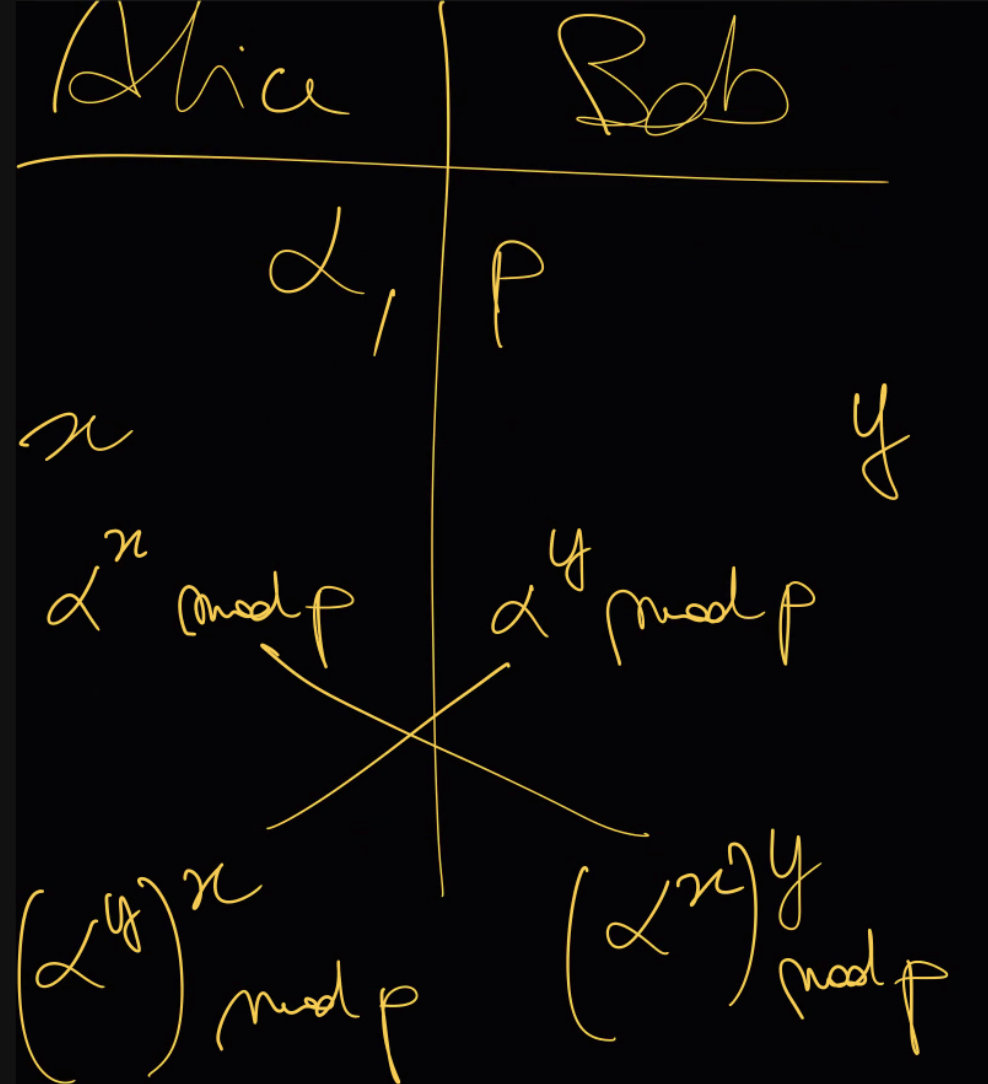
\includegraphics[scale= 0.5]{dellman}
\end{center}

\subsubsection*{Vulnerabilità di Diffie Hellman}
Consideriamo Alice, Bob ed un attaccante Eve. L'algoritmo di Diffie Hellman ci dice che:
\begin{center}
Alice spedisce $\alpha^x$ $mod$ $p$\\
Bob spedisce $\alpha^y$ $mod$ $p$\\
 \end{center}
 Consideriamo Eve che riesce a fare un attacco man in the middle:
 \begin{center}
 Eve calcola un $\alpha^z$ $mod$ $p$\\
 Eve intercetta $\alpha^x, \alpha^y$
 \end{center}
 Eve procede a inoltrare il valore tampered $\alpha^z$ ad Alice e Bob, che rispettivamente svolgono:
 \begin{center}
 Alice: $(\alpha^z)^x$ | Bob: $(\alpha^z)^y$
 \end{center}
 Eve è in grado di intercettare i due valori $x$ e $y$, e ciò gli permette di leggere e contraffare tutti i messaggi.
\begin{center}
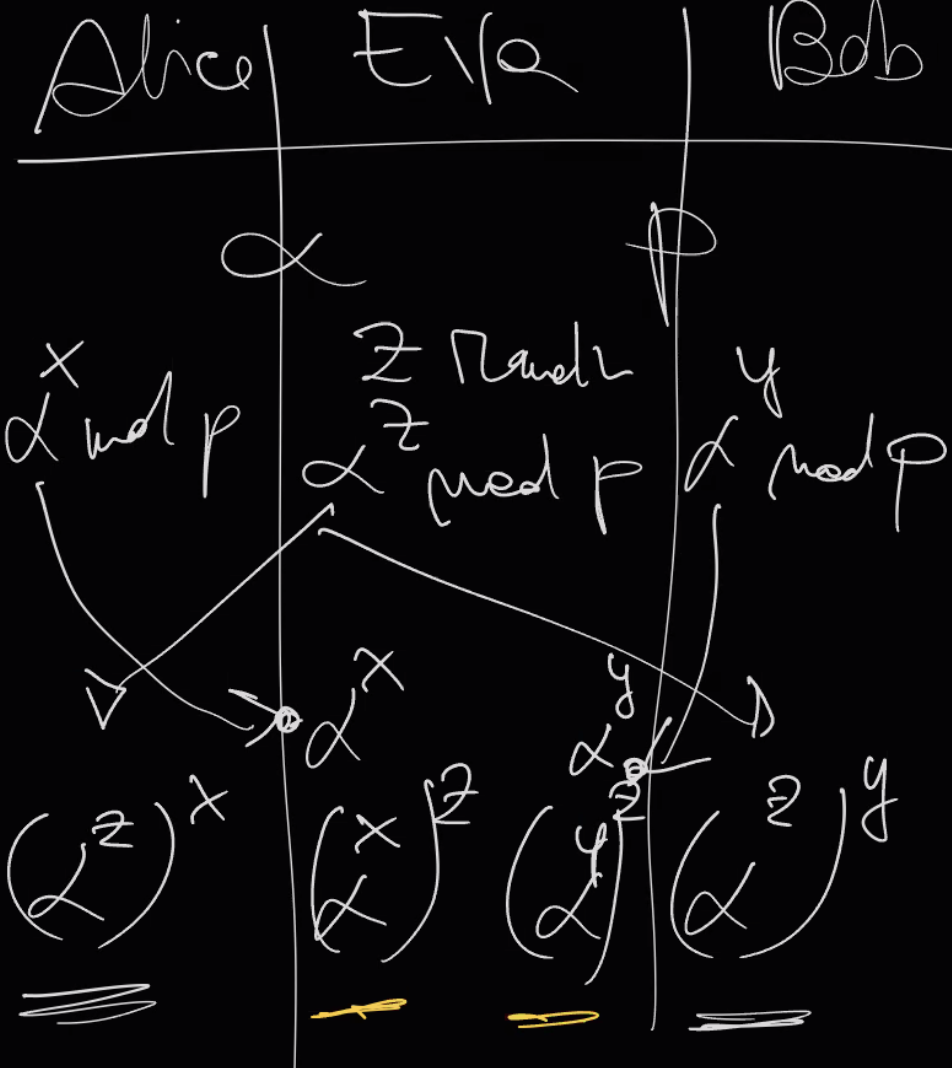
\includegraphics[scale= 0.5]{ld1}
\end{center}
Per raggirare questo problema è stato implementato STS, un sistema di firme digitali per garantire l'autenticità


\subsection*{Bit commitment}
Un'altra applicazione del logaritmo discreto l'utilizzo del bit commitment, o schema di commitment. Questo ci permette di mostrare il possedimento di un dato valore senza mostrarlo, nascondendo l'informazione all'interno del problema del logaritmo discreto. Consideriamo
\begin{center}
$\alpha^x = \beta$ $mod$ $p$
\end{center}
Se per esempio voglio inserire un'informazione all'interno del problema del logaritmo discreto, seleziono una posizione particolare all'interno di $x$, per esempio il valore del bit a posizione 1024, e gli attribuisco valore 0, se un tennista vince, e 1 se in tennista perde.\\

Inoltrando all'altra parte il valore $\beta$, possiamo essere certi di due fatti:
\begin{itemize}
\item io non sono in grado a posteriori di modificare il valore, in quanto andrebbe a cambiare fondamentalmente il problema.
\item in seguito all'evento l'altra parte può andare a verificare la posizione 1024 del valore $x$, dopo avergli fornito il valore $\alpha$, e verificare la correttezza
\item l'operazione è svolta più volte, per garantire che non sia un colpo di fortuna. Funziona similmente alle funzioni zero knowledge.
\end{itemize}

\section*{ElGamal}
E' un algoritmo di cifratura a chiave asimmetrica. Il funzionamento dell'algoritmo può essere suddiviso nelle fasi di computazione delle componenti pubbliche, pubblicazione delle componenti pubbliche, passo di cifratura, e passo di decifratura.
\subsubsection*{Computazione delle componenti pubbliche di Bob}
Bob, prima di poter utilizzare ElGamal deve selezionare una serie di parametri, in particolare:
\begin{enumerate}
\item $\alpha$ radice primitiva
\item $\phi$ o $p$ numero primo
\item $a$ numero segreto
\end{enumerate}
Con questi, Bob calcola:
\begin{center}
$\alpha^a \equiv \beta$ $mod$ $p$\\
\emph{più in particolare Bob calcola $\beta$, in quanto $\alpha$ e $\phi$ li possiede}
\end{center}
I dati $(\alpha, \phi/p, \beta)$ rappresentano la componente pubblica di Bob.

\subsubsection*{Passo di cifratura da parte di Alice}
Consideriamo ora Alice con un messaggio $m$, per cifrare il proprio messaggio: 
\begin{enumerate}
\item scarica le informazioni pubbliche di Bob $(\alpha, p, \beta)$ 
\item genera un valore $k$ casuale segreto. A partire da $k$ calcola $r,t$, in particolare:
\begin{equation}
    \begin{cases}
r = \alpha^k$ $mod$ $p\\
t = \beta^k  * m$ $mod$ $p
\end{cases}
\end{equation}
\item La coppia $(r,t)$ rappresenta il messaggio cifrato da spedire a Bob
\end{enumerate}

\subsubsection*{Passo di decifratura da parte di Bob}
Bob per decifrare effettua:
\begin{center}
$t * r^{-a} \equiv m$ $mod$ $p$
\end{center}
Stiamo incorporando il messaggio all'interno del problema del logaritmo discreto, che l'attaccante non riesce a bucare.
\subsection*{Dimostrazione di corretta di ElGamal}
Consideriamo: \begin{center}
$t * r^{-a} =$ 
\end{center}
Come abbiamo detto in precedenza $t = \beta^k  * m$ $mod$ $p$ e $r = \alpha^k$ $mod$ $p$, possiamo quindi riscrivere l'equazione nel seguente modo: \begin{center}
$(\beta^k * m)(\alpha^k)^{-a}=$
\end{center}
Ma abbiamo pure detto che $\alpha^a = \beta$, possiamo quindi riscrivere l'equazione nel seguente modo:
\begin{center}
$[(\alpha^a)^k*m]*(\alpha^k)^{-a} = $
\end{center}
Ma siccome per le proprietà delle potenze possiamo eliminare le $\alpha$, rimaniamo con:
\begin{center}
$m$ $mod$ $p$
\end{center}


\subsection*{Problematiche con ElGamal}
\subsubsection*{Valore k comune}
Consideriamo Alice con due messaggi $m_1, m_2$, cosa succede se Alice cifra due messaggi con $k$ uguale. Alice cifra ed i due messaggi derivanti sono:
\begin{center}
$(r, t_1) | (r, t_2)$
\end{center}
Siccome $r$  è una componente pubblica, l'attaccante può vedere senza problemi che Alice ha utilizzato un $k$ uguale per entrambi i messaggi, in quanto i valori $r$ sono uguali. L'attaccante conosce $t_1, t_2$, ma non i valori a destra dell'uguale:
\begin{center}
$t_1 = \beta^k * m_1$ $mod$ $p$\\
$t_2 = \beta^k * m_2$ $mod$ $p$
\end{center}
L'attaccante tuttavia sa che:
\begin{center}
$t_1/m_1 = \beta_k = t_2/m_2$
\end{center}
Può quindi computare il messaggio facendo:
\begin{center}
$m_2 = t_2  * m_1/t_1$
\end{center}

\section*{Funzioni Hash}
Una funzione hash è una funzione matematica/crittografica. Le principali caratteristiche delle funzione hash sono:\begin{itemize}
\item la facilità di computazione
\item l'input può essere una stringa di una qualsiasi dimensione
\item l'output ha una dimensione fissa, specifica per ogni funzione hash
\end{itemize}
Alcuni esempi di funzioni hash sono SHA1, SHA256, MD5, SHA3 etc.

\subsection*{Collision free property}
Una funzione di hash è perfetta se è iniettiva, ovvero se $u = v$, $h(u) \neq h(v)$, più una funzione di hash sparpaglia gli elementi, meglio è. E' tuttavia possibile che due elementi abbiamo una stessa chiave, in questo caso parliamo di $collisione$. \\
Le collisioni comportano che un output della hash function abbia 2 input medesimi. E' tuttavia possibile trovarli?
\begin{center}
\includegraphics[scale= 0.3]{h1}
\end{center}
Se vengono computati i valori hash di $2^{130}$ stringhe, la probabilità di trovare 2 valori con lo stesso output hash è del 99\%. E' tuttavia un valore cosi astronomicamente alto che è possibile considerarla nulla.\\
Possiamo quindi considerare che le funzioni hash siano collision free (non proprio, ma non importa). Concludiamo quindi che:
\begin{center}
$H(x) = H(y) \rightarrow x = y$
\end{center}

\subsection*{Pre-image resistance}
\begin{center}
\includegraphics[scale= 0.3]{h2}
\end{center}
Consideriamo un valore hash $H(x)$, è computazionalmente impossibile ricavare $x$, ovvero la funzione non è reversibile (a partire da un valore hashato, non posso risalire alla fonte). In particolare la funzione hash è chiamata one-way. Possiamo quindi concludere che per nascondere un messaggio $x$ è possibile hasharlo con $H(x)$
\subsection*{Second pre-image resistance}
\begin{center}
\includegraphics[scale= 0.3]{h3}
\end{center}
Dato un valore $x$, è computazionalmente impossibile trovare un valore $y$ tale che $H(x) = H(y)$.

\subsection*{SHA1}
SHA1 è una funzione hash crittografica che produce hash values di lunghezza 160. SHA1 lavora svolgendo 80 round della seguente funzione:
\begin{center}
\includegraphics[scale= 0.3]{sh1}\\
\emph{Ogni 20 round la funzione $f$ ed il valore $k$ cambiano}
\end{center}

\begin{itemize}
\item I blocchi A, B, C, D sono blocchi di 32 bit\\
In particolare i blocchi A, B, C, D sono inizializzati con valori in big endian con valore esadecimale in ordine crescente:
\begin{center}
\includegraphics[scale= 0.5]{blocks}
\end{center}
I valori costanti presenti nei blocchi cambiano dal passo $n_2$ in poi. Dopo 80 round di SHA1, questo output è utilizzato come valore costante iniziale per i blocchi successivi
\item $F$ è una funzione lineare
\item $<<<$ rappresenta una funzione di shift, rispettivamente di 5 e 30 posizioni
\item $W_t$ rappresenta il plaintext del round $t$, di grandezza 512 bit.\\
Consideriamo un messaggio $m$ (la divina commedia) di lunghezza $n$ ($n$ lunghezza arbitraria), il messaggio $m$ è diviso in $k$ blocchi di grandezza 512, questi 512 bit sono divisi in blocchi $W_j$ da 32 bit ciascuno.\\ In particolare se il messaggio è lungo 512 bit, questo ci produrrà 16 blocchi che rappresentano rispettivamente un valore di $W_j$ da 32 bit $(16*32 = 512)$.\\
\emph{Ma io ho bisogno di fare 79 rounds, e ne ho solo 16, cosa faccio?}
\begin{center}
\includegraphics[scale= 0.5]{blocks2}
\end{center}
Dal round 16 in poi, quindi, vengono presi 3 blocchi, e $XOR$ati tra di loro, per poi effettuare un $leftrotate$
\item $K_t$ è una costante, valore che dipende dal numero di round in cui ci troviamo
\begin{center}
\includegraphics[scale= 0.5]{blocks3}
\end{center}
\item Infine svogliamo una semplice somma per rendere SHA1 immune ad attacchi semplici:
\begin{center}
\includegraphics[scale= 0.5]{blocks4}
\end{center}
\end{itemize}

\subsection*{SHA1 | password hashing}
Consideriamo di voler hashare una password, queste essendo solitamente corte potremmo trovarci in una situazione in cui non riusciamo a riempire neanche il primo blocco $W_k$:
\begin{center}
\includegraphics[scale= 0.5]{blocks5}
\end{center}
Utilizziamo quindi un padding, in particolare vengono aggiunti un bit di $1$ ed $n$ bit $0$, in particolare $n$ fino al 448 bit. Nei rimanenti 64 bit inseriamo:
\begin{center}
\includegraphics[scale= 0.3]{blocks6}
\end{center}
In particolare il 5to ed il 4to bit da destra vengono settati ad 1 in quando la lunghezza della parola Andrea è $48 bit = 32 + 16 = 2^5 + 2^4$, ed i rimanenti bit sono settati a 0, fino a 64.
\begin{center}
\includegraphics[scale= 0.3]{blocks7}
\end{center}

\section*{On the weakness of PBKDF2 | LUKS}
Consideriamo la modalità con cui vengono salvate le password all'interno dei sistemi Linux. La definizione della funzione di hashing è importante in quanto deve trasformare una sequenza di caratteri generalmente corta, e quindi senza molta entropia, in una chiave crittografica, in grado di resistere ad attacchi di tipo brute force e dictionary. 

Entrano quindi le PBKDF, ovvero le password based key derivation functions, che data una password mi derivano un qualcosa.

\subsection*{PBKDF2}
Password Based Key Derivation Function version 2 è una key derivation function sviluppata da RSA laboratories, introduce operazioni CPU intensive, basate su un approccio iterativo pseudorandomico (ad esempio funzioni hash, cipher o HMAC).  

Una proprietà importante delle key derivation function è la "cycle free", ovvero la non-presenza di cicli determinabili o non, in quanto un potenziale attaccante se fosse in grado di riconoscerne, sarebbe in grado di saltare tale lavoro.

\subsection*{HMAC}
Il meccanismo che entra in gioco è l'HMAC o Hash-Based Message Authentication Code è un algoritmo che ci permette di generare salvare password in maniera sicura, facendo un doppio utilizzo della funzione hash.
Consideriamo:
\begin{itemize}
\item $H$: una qualsiasi funzione crittografica
\item $K$: la chiave segreta
\item $text$: l'informazione da cifrare
\item $ipad$ e $opad$ due valori costanti, rispettivamente $0x36 e 0x5C$ ripetuti 64 volte che vengono XORati con la password
\end{itemize}
\begin{center}
\includegraphics[scale= 0.5]{HMAC}\\
\emph{la password è inizialmente hashata con SHA1, che viene poi utilizzato per inizializzare il successivo blocco}
\end{center}
La sicurezza di HMAC deriva dall'impossibilità dell'attaccante di trovare una collisione sulla seconda operazione di hashing. Anche se potenzialmente fosse in grado di trovare una collisione sulla prima operazione, è sicuramente non in grado di trovarne una sulla seconda.

\subsection*{Funzionamento di PBKDF2}
La funzione HMAC è utilizzata $c$ volte, il valore $c$ dipende dalla potenza computazionale del dispositivo che sta svolgendo la funzione di encryption.
\begin{center}
\includegraphics[scale= 0.5]{pbk}
\end{center}
Questa tecnica viene utilizzata per rallentare gli attaccanti, i conti effettuati possono essere considerati "inutili, a vuoto", che tuttavia garantiscono che un attaccante sia scoraggiato dall'eseguirli.


\subsection*{Attacco a SHA1 | SHAttered: first public collision}
On 23 February 2017, the CWI (Centrum Wiskunde \& Informatica) and Google announced the SHAttered attack, in which they generated two different PDF files with the same SHA-1 hash in roughly $2^{63.1}$ SHA-1 evaluations. This attack is about $100,000$ times faster than brute forcing a SHA-1 collision with a birthday attack, which was estimated to take $2^{80}$ SHA-1 evaluations. The attack required "the equivalent processing power of 6,500 years of single-CPU computations and 110 years of single-GPU computations"

\subsection*{Attacchi a funzioni hash}
\subsubsection*{Paradosso del compleanno}
Utilizzato per attaccare le funzioni hash e le firme digitali, il paradosso afferma che la probabilità che almeno due persone in un gruppo compiano gli anni lo stesso giorno è largamente superiore a quanto potrebbe dire l'intuito: infatti già in un gruppo di 23 persone la probabilità è circa 0,51 (51\%); con 30 persone essa supera 0,70 (70\%), con 50 persone tocca addirittura 0,97 (97\%). \\
Calcoliamo la probabilità secondo la quale 23 non compiano gli anni lo stesso giorno:
\begin{center}
$PND = (1 - 1/365) * (1-2/365)*$ $...$ $(1-22/365)$
\end{center}
Se ora calcoliamo \begin{center}
$1-PND$
\end{center}
Possiamo calcolare la probabilità di collisione.\\\\
Se PND è $0,493$ allora $1 - PND = 0,507$, ovvero c'è una probabilità del 50\% che due persone abbiamo lo stesso compleanno. In particolare la probabilità è 70\% per 30 persone, 89\% per 40 persone. La probabilità della collisione è approssimabile con \begin{center}
$1 - e^{-r^2/2N}$\\
ove $N =$ dimensione del campione $(365)$\\
e $r$ = dimensione scelta $(23, 30, 40)$
\end{center}
Un altro esempio applicabile è l'analisi delle targhe delle automobili, quant'è il numero di macchine che dobbiamo esaminare perché due abbiano la porzione delle cifre uguale?
\subsubsection*{Consideriamo con le funzioni hash}
N= è il nostro digest\\
r = numero di hash che dobbiamo calcolare per trovare una collisione\\
Questo tuttavia non ci permette di attaccare SHA1, in quanto gli hash che calcoliamo noi sono randomici. Per attaccare SHA1 effettuiamo un attacco simile a baby step giant step, calcolando
\begin{center}
$P = 1 - e^-\lambda$\\
$\lambda = r^2/N$
\end{center}

\section*{Firma digitale}
La firma digitale è un schema di verifica utilizzata per garantire l'autenticità di messaggi digitali o documenti. Consideriamo un contratto con messaggio $m$, effettuiamo:
\begin{center}
$m \rightarrow hash(m) \rightarrow$ $Firma RSA(hash(m))$
\end{center}
Il crittografo in questo caso deve difendersi sia dall'attacco a $hash(m)$ che da attacchi a $Firma RSA(hash(m))$. Andiamo quindi a firmare $l'hash(m)$ con RSA, consideriamo:
\begin{center}
Public: $(n,e)$\\
Private: $(p, q, d)$
\end{center}
E procedura di encryption $m^e = c$, e procedura di decryption $c^d = m$, andiamo ad applicare una variante. Consideriamo che $d$ è la chiave privata, posseduta solo dal proprietario.\\
Consideriamo procedura di encryption $m^d = c$ e procedura di decryption $c^e = m$.
\begin{center}
$m \rightarrow hash(m) = h$\\
$h^d \rightarrow$ firma
\end{center}

\long\def\comment#1{
\subsection*{MSG recovery schemes RSA | Signatures with appendix El Gamal}
\emph{TBD to be completed}
\begin{center}
$El-Gamal: m, sig (h(m))$\\
\end{center}
}

\section*{Funzioni "zero-knowledge"}
It is common practice to label the two parties in a zero-knowledge proof as Peggy (the prover of the statement) and Victor (the verifier of the statement).\\
\begin{center}
\includegraphics[scale= 0.3]{0k}
\end{center}
In this story, Peggy has uncovered the secret word used to open a magic door in a cave. The cave is shaped like a ring, with the entrance on one side and the magic door blocking the opposite side. Victor wants to know whether Peggy knows the secret word; but Peggy, being a very private person, does not want to reveal her knowledge (the secret word) to Victor or to reveal the fact of her knowledge to the world in general.\\

They label the left and right paths from the entrance A and B. First, Victor waits outside the cave as Peggy goes in. Peggy takes either path A or B; Victor is not allowed to see which path she takes. Then, Victor enters the cave and shouts the name of the path he wants her to use to return, either A or B, chosen at random. Providing she really does know the magic word, this is easy: she opens the door, if necessary, and returns along the desired path.\\
\begin{center}
\includegraphics[scale= 0.3]{1k}
\end{center}

However, suppose she did not know the word. Then, she would only be able to return by the named path if Victor were to give the name of the same path by which she had entered. Since Victor would choose A or B at random, she would have a 50\% chance of guessing correctly. If they were to repeat this trick many times, say 20 times in a row, her chance of successfully anticipating all of Victor's requests would become vanishingly small (1 in 220, or very roughly 1 in a million).\\
Thus, if Peggy repeatedly appears at the exit Victor names, he can conclude that it is extremely probable that Peggy does, in fact, know the secret word.

\section*{Block-chaining \& Distributed Ledger Technology}
Il bitcoin ed il blockchain è un argomento strettamente legato alla crittografia e alle funzioni hash.
L'obbiettivo del bitcoin è quello di creare un sistema di scambio e verifica basato sulla crittografia, ed il bitcoin è il più grande esempio.
\begin{itemize}
\item la firma digitale per aggiungere una transazione
\item controllo e aggiunta di transazioni se e solo se la maggior parte del network lo ammette
\item sistema di remunerazione per i mantenitori del network, basato sulla scoperta di una collisione parziale all'interno del protocollo SHA2
\end{itemize}

\subsection*{Il Blockchain}
\begin{center}
\includegraphics[scale= 0.5]{bchainoverview}
\end{center}
Il blockchain rappresenta l'insieme delle transazioni svolte all'interno del network.
\begin{center}
\includegraphics[scale= 0.5]{bchain}
\end{center}
\subsection*{La validazione delle transazioni}
Per validare delle transazioni, il network lavora nel seguente modo:
\begin{enumerate}
\item un sottoinsieme del network sceglie $n$ transazioni dal paniere delle transazioni
\item viene calcolato il doppio hash delle transazioni con SHA2, utilizzando un NONCE valore casuale
\item quando viene trovato il NONCE valore corretto, il resto del network convalida l'operazione, e chi l'ha scoperto viene remunerato e i valori sono aggiunti alla blockchain
\end{enumerate}

\subsection*{Merkle-Tree}
Consideriamo una serie di transazioni, da 1 a 8, calcoliamo i loro hash, e li raggruppiamo a 2 a 2.
\begin{center}
\includegraphics[scale= 0.3]{2k}
\end{center}
I dati dei due puntatori hash vengono combinati, e utilizzati per calcolare un nuovo puntatore hash, interando progressivamente arriviamo prima o poi a una radice.
\begin{center}
\includegraphics[scale= 0.3]{3k}
\end{center}
Questo albero è chiamato un Merkle tree. Il Merkle Tree permette di verificare una potenziale manomissione, se per esempio un attaccante modifica una transazione, o un nodo intermedio, il valore della radice cambia.
\begin{center}
\includegraphics[scale= 0.3]{4k}
\end{center}
Un'altra proprietà del Merkel Tree è che ci permette di verificare l'appartenenza. Se vogliamo per esempio verificare pubblicamente che una transazione sia presente all'interno di un albero, conoscendo solo la radice, mostriamo i nodi dalla radice alla transazione.
\begin{center}
\includegraphics[scale= 0.3]{5k}
\end{center}
Questo ci permette di mostrare l'appartenenza all'albero, senza mostrare il valore della transazione.
Per effettivamente mostrare la proprietà di una transazione viene utilizzata la firma digitale.\\

\subsection*{Per riassumere}
Gli hash pointers sono strutture dati che ci permettono di costruire le strutture dati necessarie per creare una blockchain, inserire transazioni, verificare la presenza di manomissioni, e verificare l'appartenenza.

\long\def\comment#1{
Consideriamo di voler accedere alla posta di unimi:
\begin{center}
\includegraphics[scale= 0.6]{tls3}
\includegraphics[scale= 0.6]{tls4}
\includegraphics[scale= 0.6]{tls5}
\end{center}
\begin{itemize}
\item common name va a identificare il soggetto che sta utilizzando il certificato
\item issuer name va ad identificare l'ente che ha emesso la il certificato (che effettua i calcoli sui primi etc.)
\item public key info fornisce i parametri della chiave RSA 
\item i dati all'interno della connessione sono scambiati con AES o simili
\end{itemize}
Per calcolare una firma facciamo l'hash che SHA e validiamo con RSA, il fingerprint è utilizzato per garantire che il nostro certificato non sia modificato, calcolato sia con SHA1 che con SHA256, per garantire che un potenziale attaccante debba attaccare entrambi gli algoritmi.
}

\section*{SSL | TLS}
SSL è un protocollo utilizzato per scambiare informazioni su internet in maniera sicura. SSL, o Secure Sockets Layer è stato sviluppato da Netscape nel 1994 per proteggere i dati in trasferimento in rete (cartolina vs busta in rete). \\
TLS, o Transport Layer Security è stato sviluppato da Internet Engineering Task Force (IETF) è un'evoluzione di SSL, standardizzato ed utilizzabile dal pubblico.
TLS1.0 (99), inizialmente praticamente uguale a SSL3 ('96), viene poi aggiornato in TLS1.1 ('06), TLS 1.2 ('08), TLS1.3 ('18). Ogni aggiornamento va a migliorare la sicurezza e l'interoperabilità.\\

SSL e TLS durante la connessione producono \emph{session states e connection states}, informazioni che vengono scambiati attraverso il processo descritto dal protocollo di handshake per concordare i protocolli/parametri da utilizzare durante la connessione.
\begin{center}
\includegraphics[scale= 0.6]{tls}\\
\emph{5: Diffie-Hellman}
\end{center}
Dopo la terminazione del processo di handshake il client ed il server sono pronti a scambiare informazioni in base ai parametri che si sono appena condivisi.\\
All'interno del protocollo sono presenti una serie di campi, ad esempi l'alert protocol che va ad informare l'utente di eventuali problemi minori (no, revoked, expired certificates) e grandi (bad record MAC (connection tampering), handshake failure, illegal parameter).

\section*{Curve elittiche}
Le curve elittiche sono adottate perché, a parità di grandezza delle chiavi, garantiscono un ordine di grandezza più sicurezza (4000 bit RSA vs 300 bit EC). Questo ci permette di risparmiare sulla grandezza delle chiavi, velocizzando i calcoli. (Il livello di sicurezza è uguale, è solo che con RSA mi servirebbe una chiave più lunga).

\begin{center}
\includegraphics[scale= 0.6]{curves}\\
\emph{esempio di curve ellittiche}
\end{center}
Una curva ellittica come la studiamo noi è rappresentata da una funzione, in particolare:
\begin{center}
$y^2 = x^3 + ax^2 + bx + c$\\
$a, b, c \in Insieme$
\end{center}
Ove per $Insieme$ si intende un insieme finito, in particolare un campo $K$ finito chiamato $Z_5$ in modulo $p$. Una curva ellittica rappresenta l'insieme dei punti geometrici che risolvono l'equazione.
In particolare l'insieme delle soluzioni di una curva ellittica è la seguente:
\begin{center}
$S = \{(x,y)$ ove $x, y \in K$ e $y^2 = x^3 + ax^2 + bx + c\}$
\end{center}
Quando tuttavia le trattiamo noi, le tratteremo in termini di campo (in questo caso $Z_5$) ad esempio:
\begin{center}
$y^2 = x^3 + 2x -1$ $mod$ $5$
\end{center}


\subsection*{Punto all'$\infty$ o punto $O$}
Il punto all'infinito è un punto speciale in ogni curva ellittica, è rappresentata dall'intersezione delle rette parallele all'asse $y$ in prospettiva.
\begin{center}
\includegraphics[scale= 0.4]{pzero}
\end{center}

\subsection*{Legge dell'addizione e la somma di punti}
Consideriamo $P_1, P_2, P_3$, e $P_1 + P_2 = P_3$ questa operazione è svolta nel seguente modo:
\begin{center}
\includegraphics[scale= 0.4]{curva}\\
\emph{calcolo prima $Q$, e $P_3$ è ricavato negando l'$y$}
\end{center}
\begin{itemize}
\item costruiamo la retta che passa passante per $P_1$ e $P_2$
\item il punto in cui interseca nuovamente la curva è chiamato $Q$
\item calcolo la perpendicolare rispetto all'asse $x$ che passa dal punto $Q$, quando nuovamente incontra la curva abbiamo trovato $P_3$
\end{itemize}
Matematicamente l'operazione di calcolare $Q$ è svolta facendo il sistema tra la curva, e la retta che passa per $P_1$ e $P_2$
\begin{equation}
    \begin{cases}
y^3 = x^3 + ax^2 + bx + c\\
y = mx + q
\end{cases}
\end{equation}
Dobbiamo tuttavia considerare i casi particolari, ad esempio il caso in cui $P_1$ e $P_2$ siano identici, in questo caso la retta passante sarà semplicemente la tangente. \\
Un altro caso da considerare è quello in cui la retta passante è parallela all'asse $y$, in questo caso $P_3$ sarà il punto all'$\infty$\\

Altre proprietà delle curve ellittiche sono:
\begin{itemize}
\item $P + \infty = P$
\item $P - (x, y ) = P + (x, -y)$
\item la commutatività: $P + Q = Q + P$
\item l'associatività: $(P + Q) + R = P +  (Q + R)$
\end{itemize}
Ma se siamo in grado noi di calcolare i punti, lo può fare anche un attaccante. Dal punto di vista crittografico dobbiamo andare a rafforzare il cifrario, in particolare facciamo due cose:

\subsection*{Utilizziamo l'equazione ed il valore $p$ adatto}
Consideriamo una curva standard:
\begin{center}
$y^3 = x^3 + ax^2 + bx + c$ $mod$ $p$
\end{center}
Nel mondo reale il valore $p$ è un valore grande, dell'ordine di grandezza $10^{100}$. Questo è fatto perché obbliga un potenziale attaccante a provare tutti i valori da 1 a $10^{100}$.\\

Dobbiamo inoltre accennare che quando le curve ellittiche vengono utilizzate nel mondo reale, solo un piccolissimo sottoinsieme vengono utilizzate, studiate appositamente perché non siano attaccabili.

\subsection*{Incorporiamo il problema del logaritmo discreto}
incorporiamo il problema del logaritmo discreto. Ricordiamo:
\begin{center}
$\alpha^x \equiv \beta$ $mod$ $p$
\end{center}
Il valore all'esponente $x$ è utilizzato come numero di volte per sommare il punto $P$ di interesse, in particolare va $x$ a rappresentare il numero di volte che dobbiamo sommare il punto.
\begin{center}
$(P_1 + ...  + P_1) $ ove $n = x$
\end{center}

\subsection*{Funzionamento nel mondo reale}
Svolgere l'operazione di calcolo del punto $P_3$ nel modo canonico è un'operazione dispendiosa, andiamo quindi a considerare dei calcoli più diretti.\\
Consideriamo $P_1 = (x_1, y_1), P_2 = (x_2, y_2), P_3 = (x_3, y_3)$
\begin{itemize}
\item $P_1 + P_2 = P_3$
\item $x_3 = m^2 - x_1 - x_2$ 
\item $y_3 = m(x_1 - x_3) - y_1$
\item $m$ è il coefficiente angolare della retta passante per $P_1$ e $P_2$
\end{itemize}
Ci manca solo $m$, che possiamo calcolare in 2 modi a seconda del caso:
\begin{itemize}
\item se $P_1  \neq P_2$ allora $(y_2 - y_1)/(x_2 -x_1)$
\item se $P_1 = P_2$ allora $(3x_1^2 + b) / 2y_1$
\end{itemize}

\subsection*{Esempio di codifica}
Consideriamo un messaggio, ad esempio "ciao". Il messaggio è codificato in un numero secondo un criterio (uno qualsiasi, ad esempio ASCII). Il messaggio codificato viene inserito in un punto nella curva ellittica. \\

Dobbiamo tuttavia notare che non tutti i punti $x$ della curva ellittica possiede un corrispettivo $y$, in questi casi adottiamo un algoritmo probabilistico chiamato algoritmo di Koblitz

Consideriamo:
\begin{itemize}
\item $mod$ $p$ = 179
\item EC: $y^2 = x^3 + 2x + 7$ 
\item Messaggio $m$ = 5 ("C" nella nostra parola "Ciao")
\end{itemize}

\subsubsection*{Algoritmo di Koblitz}
E' un algoritmo probabilistico che ci permette di gestire numeri che normalmente non sono utilizzati nelle curve elittiche. Fissiamo un valore $k$ che sta a rappresentare una soglia (probabilità di errore).
Il valore $k = 1/2^k$ è la probabilità di errore. \\
Supponiamo di fissare $k = 10$, eseguiamo la seguente operazione:
\begin{center}
$m * k + k < p$
\end{center}
Nel nostro esempio 
\begin{center}
$m * 10 + 10 < 179$\\
\end{center}
Questo ci dice che possiamo rappresentare tutti i valori che sono compresi tra 0 e 16:
\begin{center}
$0 \leq m \leq 16$ $\rightarrow$ $m = 5 \leq 16$
\end{center}
Che diventa utilizzabile nella nostra curva ellittica, il valore $x$ è quindi rappresentato da 
\begin{center}
$x = m * k  + j$
\end{center}
Il valore $j$ è un valore compreso tra $0 \leq ... \leq j$ over $j = k - 1$

Nel nostro esempio abbiamo $5 * 10 + j$, $t * 10 +0 = 50$, quindi $x = 50$. Questo valore è quindi utilizzabile dentro all'equazione della curva ellittica, che quindi diventa
\begin{center}
$y^2 = 50^3 + 2*50 + 7$ $mod$ $179$
\end{center}
Possiamo risolvere la funzione, facendo $y^2 = 165$, troviamo tuttavia che non esiste un $y$ valido.\\
Quando non troviamo un $y$ valido, andiamo a provare con un $j$ diverso, normalmente il valore successivo.\\\\
Svolgiamo quindi $5 * 10 +1 = 51$, che ci da $x = 51$. L'equazione della curva ellittica diventa quindi
\begin{center}
$y^2 = 51^3 + 2*51 + 7$ $mod$ $179$ 
\end{center}
Ed in questo caso il la funzione è risolvibile con $y^2 = 121$ e la coppia è $(51, 11)$.
La coppia va a rappresentare il messaggio $m$, codificato con la curva ellittica. 

\subsubsection*{La componente probabilistica}
La componente probabilistica entra in gioco in relazione al campo, e al valore $k$ fissato all'inizio. La probabilità di trovare un valore $j$ adatto da inserire è strettamente legato al valore $k$, che rappresenta anche il numero di tentativi massimi.\\

Per ricavere il messaggio iniziale svolgiamo l'operazione inversa $m = x/k$, in questo caso $51/10 = 5(,1)$. Il valore non è precissimo, possiamo infatti vedere che tutti i valori da 50 a 59 sarebbero validi, questo dipende strettamente dal valore $k$. 

\subsection*{Teorema di Hasse}
Consideriamo una EC $mod$ $p$, con $N$ punti, l'algoritmo di Hasse dice che vi è una relazione tra $p$ e $N$, infatti:
\begin{center}
$|N - p - 1| < 2\sqrt p$
\end{center}
Questo ci permette di dire un pò di cose, considerando una curva ellittica $mod$ $p$
\begin{itemize}
\item N sarà dell'ordine di grandezza di $p$ ovvero $N \sim p$, 
\item Il numero di soluzioni è dato da $p/2$ numeri positivi, $p/2$ numeri negativi, ed $1$ (il punto all'$\infty$. Il totale delle soluzioni di una qualsiasi curva ellittica è quindi rappresentata da $p/2 + p/2 + 1$\\.
\end{itemize}

\subsection*{ECDH: Elliptic Curve Diffie Hellman}
\begin{center}
\includegraphics[scale= 0.3]{ecdh}
\end{center}
\begin{itemize}
\item i numeri $N_a, N_b$ sono due numeri generati casualmente.
\item $G$ rappresenta il numero del problema delle curve ellittiche da sommare per sé stesso, $N_a$ volte
\item Con i valori scambiati, Bob e Alice possono utilizzarli come seed per una KGF, in quanto l'informazione riguardo al valore delle chiavi non è passato sul canale in chiaro.
\end{itemize}
Dobbiamo accennare che nuovamente questo schema di scambio di chiavi è vulnerabile ad una attacco MITM.


\subsection*{Elliptic curve to attack RSA}
Consideriamo EC $mod$ $p$, se facessimo:
\begin{center}
EC $mod$ $n$ ove $n = p * q$ è la chiave pubblica di RSA
\end{center}
Cosa cambierebbe? Cambierebbe che quando lavoriamo con le curve ellittiche abbiamo imposto di lavorare su un campo, ma se lavoriamo su un $n$ di RSA lavoriamo su un anello.\\
Come abbiamo visto in precedenza su un campo \emph{tutti} i valori hanno un inverso moltiplicativo, ma lo stesso non può essere detto su un anello. Questo implica che non sempre è possibile effettuare la divisione per ricavare $m$ ($m$ coefficiente angolare della retta).\\

Questo problema, tuttavia ci torna utile, come abbiamo visto, l'inverso moltiplicativo è unico quando lavoriamo con $p$ se e solo se
\begin{center}
$MCD(denominatore, p) = 1$
\end{center}
Quando tuttavia andiamo a lavorare con $n$ e quindi:
\begin{center}
$MCD(denominatore, n) = 1$
\end{center}
Nel 99\% dei casi il denominatore ed $n$ sono coprimi, c'è tuttavia una bassa ma non trascurabile percentuale di casi in cui:
\begin{center}
$MCD(denominatore, n) \neq 1$
\end{center}
Come sappiamo da RSA, tuttavia, $n = p * q$, e se $MCD(denominatore, n) \neq 1$, il valore sarà uguale a $d$, che corrisponde a o $p$ o $q$. Il calcolo dell'altro parametro diventa quindi triviale.

Questo attacco, come abbiamo detto, è possibile solo nel caso in cui riusciamo a trovare un denominatore problematico, per cui non riusciamo a calcolare l'inverso moltiplicativo, perché ciò implica che il risultato corrisponderà ad uno dei fattori di $n$.
\begin{enumerate}
\item Abbiamo trovato un valore per cui vale $MCD(denominatore, n) \neq 1$
\item Che vuol dire che abbiamo trovato un valore per cui non esiste l'inverso moltiplicativo
\item Che vuol dire che abbiamo trovato uno dei termini di $n$
\end{enumerate}

\subsection*{E nel mondo reale?}
Nel mondo reale, prima di selezionare il punto $P$ di interesse andiamo a fare le verifiche, questo viene fatto sommando più volte il punto, fino a quando troviamo un valore per cui non riusciamo a calcolare l'inverso moltiplicativo, e quindi attaccabile:
\begin{center}
$P + P + ... $ 
\end{center}
Ma quante volte dobbiamo sommare $P$ prima di trovare un denominatore problematico?
Creiamo una variabile $m$ che rappresenta il più piccolo numero di volte che dobbiamo sommare $P$ per sé stesso prima di trovare un problema.

Cosa possiamo intuire di $m$?
\begin{itemize}
\item $m$ sicuramente divide $N$, ove $N$ è il numero di punti della curva ellittica in particolare $N/m = k$, $N$ è divisibile per $m$.\\ Ricordiamo che $N$ è un numero finito, in quanto in crittografia noi lavoriamo su un campo/anello.
\end{itemize}
\subsubsection*{Numero liscio e B-liscio}
Un numero liscio è un numero che è che fattorizzabile in un prodotto di numeri primi piccoli. La terminologia "B-liscio" è utilizzato per definire una soglia dei fattori, diciamo quindi che un numero è B-liscio se i numeri primi sono minori del valore $B$. 
\begin{itemize}
\item quando andiamo a selezionare un valore $N$ di ordine di grandezza $10^{300}$, la probabilità che il numero sia liscio o b-liscio non è trascurabile.
\end{itemize}
Ed un numero b-liscio è facilmente fattorizzabile.

\subsection*{Cosa possiamo fare allora?}
\begin{enumerate}
\item selezioniamo una curva ellittica a caso, ad esempio:
\begin{center}
$y^2 = x^3 + bx + c$ 
\end{center}
\item selezioniamo un punto $P$ a caso
\begin{center}
$P(0,0)$
\end{center}
\end{enumerate}
Per imporre che la curva elittica passi per il punto P, possiamo fare la sostituzione, in particolare:
\begin{center}
$0^2 = 0^3 + 0 +c$
\end{center}
e impostiamo un sistema in cui:
\begin{equation}
    \begin{cases}
a = 0\\
b = 7 $ un numero casuale$\\
c = 0 $ come da risoluzione della sostituzione$
\end{cases}
\end{equation}
Inseriamo i dati che abbiamo appena calcolato nella funzione della curva ellittica, modulando a $n$ di RSA:
\begin{center}
$y^2 = 7x$ $mod$ $n$
\end{center}
Non siamo tuttavia in grado di determinare la natura di $N$ dato che l'abbiamo determinato casualmente, diamo per scontato che sia liscio.\\

Noi sappiamo che $m * P \rightarrow \infty$, è intuibile che anche i multipli di $m * P$ tendano all'infinito, ad esempio $2m * P \rightarrow \infty$, $3m * P \rightarrow \infty$, $10!m * P \rightarrow \infty$. Siccome non riusciamo a calcolare direttamente $m$, cerchiamo un valore con cui moltiplicare $m$ per trovare la problematica.\begin{center}
$100.000! * P $
\end{center}
Se $100.000! * P $ è un multiplo di $m$, allora anche $100.000! * P $ farà andare la curva all'infinito, avremo quindi trovato un valore accettabile.\\
Questo avviene perché $N$ è liscio, e se $m$ divide $N$, anche $m$ è liscio, e $100.000!$ contiene tutti i fattoriali piccoli.
\subsubsection*{E se cosi non fosse?}
Andiamo a provare con altri parametri nella nostra curva ellittica, modificando a piacimento il punto $P$, e il parametro $b$.

\end{document}  